\documentclass[unicode,master]{scutthesis} % 草稿封面,硕士则添加选项master,博士则去掉。使用正式封面时注释该行
% \documentclass[unicode,master,pdfcover]{scutthesis} %   % 论文正式封面,pdfcover为可选项,终稿再添加,使用草稿封面时注释该行
\usepackage{fontspec,color,array,longtable,graphicx} 
\usepackage{anyfontsize} %消除字体警告
\usepackage{enumitem}
\usepackage{amsmath}
%%%%%%%%%%%%%%%%%%%%%%%%%%%%%%%%%%%%%%%%%%%%%%%%%%%%%%%%%%%%%%%%%%%%%%%%%%%%%%%%%%——by MCH
%编译范围
% \includeonly{chapter04}
%参考文献设置
\usepackage[backend=biber,style=gb7714-2015,gbalign=gb7714-2015,gbpub=false,gbnamefmt = lowercase]{biblatex}
\addbibresource[location=local]{MyLibrary.bib} % 如果在其他盘,改为相对路径。比如F盘,改为:F/MyLibrary.bib
\addbibresource[location=local]{mybibfile2.bib} % 无论什么来源的bib文件,只要由参考文献的BibTeX组成,都可以使用此模板。参考文献的BibTeX获取方法可百度
%页眉页脚设置
\addbibresource[location=local]{mtzbib.bib}
%这是我使用的文献引用%
\usepackage{fancyhdr}
\usepackage{listings}
\usepackage{xunicode}
\newcommand{\etal}{\textit{et al}.}

\renewcommand{\lstlistingname}{列表}
\pagestyle{fancy}
\fancyfoot[C]{\headfont\thepage}
\renewcommand{\chaptermark}[1]{\markboth{\chaptername\ #1}{}}
\renewcommand{\sectionmark}[1]{\markright{\thesection\ #1}}
\fancyhead[RE]{}
\fancyhead[RO]{}
\fancyhead[LE]{}
\fancyhead[LO]{}
\fancyhead[CO]{\headfont{\leftmark}}
\fancyhead[CE]{\headfont{华南理工大学硕士学位论文}}% 
\renewcommand{\headrulewidth}{1.5pt}
\renewcommand{\footrulewidth}{0pt}
%%%%%%%%%%%%%%%%%%%%%%%%%%%%%%%%%%%%%%%%%%%%%%%%%%%%%%%%%%%%%%%%%%%%%%%%%%%%%%%%%%
\usepackage[unicode=true,bookmarks=true,bookmarksnumbered=true,bookmarksopen=false,breaklinks=false,pdfborder={0 0 1},backref=false,colorlinks=true]{hyperref}
\hypersetup{pdftitle={基于渐进式策略的人体运动姿态预测算法},
	pdfauthor={马铁铮},
	pdfsubject={华南理工大学硕士学位论文},
%%	pdfsubject={华南理工大学博士学位论文},
	pdfkeywords={PDF关键字1;PDF关键字2},
%%		linkcolor=black, anchorcolor=black, citecolor=black, filecolor=black, menucolor=black, urlcolor=black, pdfstartview=FitH}% 黑白,提交版
	linkcolor=blue, anchorcolor=black, citecolor=red, filecolor=magenta, menucolor=red, urlcolor=magenta, pdfstartview=FitH}% 彩色

\makeatletter
%%%%%%%%%%%%%%%%%%%%%%%%%%%%%% LyX specific LaTeX commands.
\providecommand{\LyX}{\texorpdfstring%
	{L\kern-.1667em\lower.25em\hbox{Y}\kern-.125emX\@}
	{LyX}}
%% Because html converters don't know tabularnewline
\providecommand{\tabularnewline}{\\}
\makeatother
\begin{document}
	%%%%%%%%%%%%%草稿封面设置%%%%%%%%%%%%%使用“正式封面”时不需要理会这部分
	\title{基于渐进式策略的人体运动姿态预测算法}	
	\author{马铁铮}	
	\supervisor{指导教师:聂勇伟\ 副教授}	
	\institute{华南理工大学}	
	\date{2023年5月20日}
	%%%%%%%%%%%%%%%%%%%%%%%%%%%%%%%%%%%%%
	\maketitle	
	\frontmatter	%此后为罗马数字页码,页面类型为plain
	\chapter{摘\texorpdfstring{\quad}{}要}
	3D人体运动姿态预测(3D Human motion prediction)指:在3D空间中,根据历史人体运动姿态序列,预测未来的人体运动姿态序列。随着人工智能化浪潮的到来,该技术被广泛应用于自动驾驶、监控视频异常检测、人体动作捕捉生成等领域中,有着良好的应用前景和研究价值。例如在自动驾驶算法中,需要根据行人当前运动轨迹来预测其未来运动趋势,进而指导自动驾驶程序做出相应处置。
	
	本文提出了一种新颖的3D人体运动姿态预测算法,与现有方法相比,本方法在预测精确度和运行效率的综合指标上有大幅领先。目前现有方法大多使用单个网络直接预测未来运动姿态。由于输入人体运动姿态序列与未来人体运动姿态序列之间普遍存在较大的差异。使用单阶段网络直接预测时,往往出现模式坍塌、预测失准等情况。本文提出了一种新颖的渐进式多阶段网络,将直接预测拆分为多阶段预测,允许神经网络逐步学习复杂的人体结构特征和关节点运动模式。具体的,本文设计了一种被称为累积均值平滑(Accumulate average smooth,AAS)的中级监督目标构造方法,通过平滑关节点运动轨迹,在保留人体空间结构信息的同时,降低了关节点运动的复杂度。凭借AAS,可以在由浅至深的各个网络阶段,构造由易到难、平滑过渡的预测目标。允许网络逐步完善预测结果。另外,网络中的特征提取模块也对预测精确性有较大影响。现有方法大多使用卷积神经网络(Convolutional Neural Network,CNN)、循环神经网络(Recurrent neural network,RNN)、图卷积网络(Graph Convolutional Network,GCN)。在人体运动姿态问题中,输入数据同时包含具有空间拓扑结构的人体姿态和时间序列上的关节点轨迹。图卷积网络以其对空间拓扑数据的优秀建模能力得到了广泛的关注。但目前仍然缺乏一种同时对时空维度进行高效建模的特征提取方法。为此,我们提出了一种具有时空信息捕捉能力的图卷积,被称为ST-DGCN,该图卷积由空间和时间两部分构成,分别称为S-DGCN(Spatial \ Dense \ Graph \ Convolution)和T-DGCN(Temporal \ Dense \ Graph \ Convolution), 两部分串行组合,当运动序列输入后,首先由S-DGCN提取空间信息,随后送入T-DGCN提取时间信息,由此网络间接地捕捉了时空信息,并具有全局感受野。
		
	在渐进式结构和S-DGCN、T-DGCN这两个策略的帮助下,本方法在Human3.6M、CMU-MoCap、3DPW这三个公开数据集上使用公开度量指标,预测精度较现有方法均有较大提升,且运行效率无显著落后。


\keywordsCN{3D人体运动姿态预测、渐进式策略、时空序列、图卷积网络}

\chapter{Abstract}
3D human motion prediction refers to predicting the future human motion sequence in 3D space based on the historical human motion posture sequence. With the arrival of the AI wave, this technology has been widely used in fields such as autonomous driving, abnormal detection in surveillance videos, and human motion capture generation, with good application prospects and research value. For example, in autonomous driving algorithms, it is necessary to predict the future movement trend of pedestrians based on their current motion trajectory, and then guide the autonomous driving program to make corresponding arrangements.

This article proposes a novel 3D human motion prediction algorithm, which outperforms existing methods in terms of prediction accuracy and operational efficiency. Currently, most existing methods use a single network to directly predict future motion postures. However, due to the significant difference between the input human motion posture sequence and the future human motion posture sequence, pattern collapse and prediction errors often occur when using a single-stage network for direct prediction. This article proposes a novel progressive multi-stage network that splits direct prediction into multiple stages, allowing the neural network to gradually learn complex human structure features and joint motion patterns. Specifically, this article designs an intermediate supervision objective construction method called Accumulate Average Smooth (AAS), which smoothes joint motion trajectories while retaining human spatial structural information and reducing joint motion complexity. With AAS, smooth transition prediction targets from easy to difficult can be constructed at each network stage, allowing the network to gradually improve the prediction results. Additionally, the feature extraction module in the network also has a significant impact on prediction accuracy. Most existing methods use Convolutional Neural Networks (CNN), Recurrent Neural Networks (RNN), and Graph Convolutional Networks (GCN). In the problem of human motion posture, the input data contains both human posture with spatial topological structure and joint trajectory on the time sequence. GCN has received widespread attention for its excellent modeling capability of spatial topological data. However, there is still a lack of feature extraction methods that efficiently model both temporal and spatial dimensions. Therefore, we propose a graph convolution with the ability to capture spatiotemporal information called ST-DGCN, which consists of two parts: S-DGCN (Spatial Dense Graph Convolution) and T-DGCN (Temporal Dense Graph Convolution). These two parts are combined in series. When the motion sequence is input, the spatial information is first extracted by S-DGCN, and then the temporal information is extracted by T-DGCN, indirectly capturing spatiotemporal information and having a global receptive field.

With the help of the progressive structure and the two strategies of S-DGCN and T-DGCN, this method improves the prediction accuracy compared to existing methods on three public datasets: Human3.6M, CMU-MoCap, and 3DPW, using public metrics, while maintaining operational efficiency.

\keywordsEN{3D human motion prediction、Progressive learning、Spatiotemporal sequence、Graph Convolutional Networks} % 中英文摘要
	%%%%%%%%%%%%%%%%%%%%%%%%%%%%%%%%%%%%%%%%%%%%%%%%
	% 目录、表格目录、插图目录这几个字本身的大纲级别是一级的,即和章名有相同的字号字体。目录表的内容通过titletoc宏包在。cls文件设置了。
	%\cleardoublepage % pdfbookmark可能需要这一条才能正常工作
	\pdfbookmark{\contentsname}{toc} %为目录添加pdf文件书签
	\tableofcontents	%目录
	% \listoffigures	%插图目录(可选)
	% \listoftables	%表格目录(可选)
	
	\begingroup
		\renewcommand*{\addvspace}[1]{}
		\newcommand{\loflabel}{图} 
		\renewcommand{\numberline}[1]{\loflabel~#1\hspace*{1em}}	
		\listoffigures
		
		\newcommand{\lotlabel}{表}
		\renewcommand{\numberline}[1]{\lotlabel~#1\hspace*{1em}}
		\listoftables
	\endgroup

	%%%%%%%%%%%%%%%%%%%%%%%%%%%%%%%%%%%%%%%%%%%%%%%%%
	% \include{symbols}	% 符号对照表(可选)
	% \include{abbreviation} 	% 缩略词	
	
	\mainmatter %此后为阿拉伯数字页码
	
    %%%%%%%%%%%%%%%%%%%%%%%%%%%%%%%%%%%%%%%%%%%%%%页眉页脚设置 ——by MCH 
    \fancypagestyle{plain}{
    	\pagestyle{fancy}
    }	% 每章的第一页会默认使用plain,没有页眉。通过重定义plain为fancy解决
    \pagestyle{fancy}	%设置页眉页脚为fancy
    %%%%%%%%%%%%%%%%%%%%%%%%%%%%%%%%%%%%%%%%%%%%%%分章节,结合导言区的\includeonly命令可仅编译部分章节,编译时不用切换界面,直接在相应章节编译即可。
	\chapter{绪论}
%
\section{研究背景和意义}
\label{section:1.1}
%研究背景
近年来随着人工智能技术和社会经济的高速发展,大量信息化、智能化的新技术渗透到了人们的日常生活中。其中理解和预测人体运动的相关研究获得了显著的进展。该技术被广泛应用于自动驾驶、智能机器人、人机交互和多媒体领域。在自动驾驶领域,车载计算机需要预测其他交通参与成员的行动意向和未来位置,并以此来规划车辆未来运行路线。在智能机器人领域,特别是用于协助人类的机器人,如工业机器人、看护机器人等,需要准确地预测人的未来运动来采取对应行动。在人机交互领域,在人口稠密的空间中,机器应准确预测周围的人的动作以安全地穿过人群。在多媒体领域,特别是游戏和影视制作场景中,和通过昂贵的动作捕捉设备获得人体运动姿态模型相比。基于软件的理解和预测人体运动方法更加廉价高效。综上,理解和预测人体运动算法在促进国民经济发展和推动数字化、智能化转型方面有重要的积极作用。意味着该课题有较高的研究潜力和应用价值。

%现阶段的研究和问题
目前学术界和工业界对该课题进行了较为细致且充分的研究。3D人体运动姿态预测问题被定义为:在某个三维场景下,已知某个个体的一段历史运动序列,算法需要根据该段历史运动中包含的趋势或规律,预测该个体在未来的运动序列。该问题的研究重点包含两部分,第一是通过对历史运动序列的理解,提取其中包含的运动信息。例如在观看任意一段运动序列后,人类可以轻易地判别出该序列的运动类型(如行走、拾取物品、舞蹈等)。但对计算机来说,如何理解运动序列中的时序信息是研究的重点。第二是基于对历史运动中时空信息的提取,预测未来运动序列。由于人体运动的高度复杂性和不确定性,如何基于有限的运动信息尽可能降低预测过程的不确定性,进而输出准确的未来运动序列,是当前研究种的一个主要难点。

%当前的研究进展
在早期的研究中,由于循环神经网络\parencite{zaremba2014recurrent}可以利用其内部隐状态(Hidden state)来捕捉输入数据中的时序依赖性,有利于处理时间序列这类序列化数据,RNN被用来提取人体运动序列中的时序信息,进而预测未来的运动序列。

这类方法的主要思路是,每个RNN Unit中的隐状态,可以根据当前的输入的人体运动姿态和上一阶段的隐状态进行更新。该隐状态是对网络过去所见信息的总结,并被用来对未来进行预测。借助节点中的隐变量的记忆和更新能力,RNN可以感知输入序列化信息中的时序依赖性。这使得RNN可以提取人体运动序列中的时序信息,高效应用于未来序列的预测任务。

然而,由于RNN中每一步输出只与当前输入和上一步隐状态有关,无法对连续的输出结果进行整体上的一致性约束。输入序列和预测序列的过渡部分会出现不连续的情况。为此,现有方法提出了一种有着编码器-解码器结构的序列到序列的网络模型(Sequence-to-Sequence),编码器将输入数据整体映射到隐空间,随后由解码器一次性预测未来运动序列。以此便可以对输出进行全局一致性约束。除了过渡部分不连续的问题,由于隐状态容量有限,RNN只能对短期依赖性进行建模,无法处理长距离时序依赖。为了解决这个问题,出现了长短期记忆\parencite{shi2015convolutional}(Long Short-Term Memory,LSTM)和门控循环单元\parencite{cho2014learning}(Gate Recurrent Unit,GRU)网络,但它们更加复杂,带来了更多的运行开销。
同时,该类方法通常将人体姿态作为一个整体输入RNN Unit,忽略了人体姿态的空间结构。然后,对于人体运动序列预测问题,人体姿态的空间结构是一个重要的先验信息。这导致基于RNN的方法在预测结果真实性和准确性方面有所欠缺。

近年来随着对图卷积网络\parencite{kipf2016semi}的深入研究,部分现有方法引入图卷积网络对人体姿态空间结构进行建模。对于人体姿态这类不规则图状数据,图卷积网络有着天然的优势。在这类方法中,人体姿态被视作由节点集合和连接顶点的边集合组成的数据结构。图卷积网络借助拉普拉斯矩阵描述关节点之间的信息流动状态,进而对复杂的节点对间的关联进行建模。但传统图卷积网络主要应用于二维平面数据结构。如何设计高效的,具有时空信息提取能力的图卷积网络,对于人体运动序列预测这类涉及时空序列数据的问题尤为重要,至今也依旧是学术界的一个难点问题。

除了需要有效提取输入序列中的时空信息,如何降低预测过程中的不确定性也是需要考虑的问题。在大多数情况下,由于人体运动序列的复杂性,输入序列和未来序列之间存在较大的差异,这导致预测过程存在较大的不确定性和预测歧义。现有方法大多采用单个前馈神经网络,接受历史运动序列,随后直接预测未来运动序列。在这一过程中,网络将承受较大的不确定性,预测结果可能出现模式坍塌(Mode collapse)和预测失准等问题。因此,设计更高效的预测策略来降低预测过程中的不确定性和歧义,是当前研究中需要重视的另一个问题。

%我们的贡献
\section{主要研究内容及贡献}
针对上述研究存在的问题和人体运动姿态预测问题的特点,本文主要的研究内容和贡献被总结如下:

1.基于渐进式策略的人体运动姿态预测算法框架。
\begin{enumerate}[topsep = 0 pt, itemsep= 0 pt, parsep=0pt, partopsep=0pt, leftmargin=44pt, itemindent=0pt, labelsep=6pt]
	\item[$\bullet$] 与现有方法使用单阶段的网络结构不同,本文将预测过程拆分为多个阶段,除开位于网络入口的阶段,其他阶段均在上一步预测基础上进行预测,这将有利于降低每一阶段的预测难度。
	\item[$\bullet$] 本文遵循网络由浅至深,预测难度由易到难的原则。浅层阶段只负责预测大致的运动趋势,复杂的运动细节预测则由具有深层语义提取能力的深层阶段负责。
	\item[$\bullet$] 为了构建多阶段、渐进式的网络,本文为每个阶段构造对应的中级监督目标(Intermediate target)。具体的,本文设计了一种人体运动轨迹平滑方法,通过平滑关节点运动轨迹的方式,去除运动细节,为每个阶段提供不同平滑程度的预测目标。
\end{enumerate}

2.具有时空信息提取能力的Spatiotemproal 图卷积网络模块(S−DGCN 和 T−DGCN)。
\begin{enumerate}[topsep = 0 pt, itemsep= 0 pt, parsep=0pt, partopsep=0pt, leftmargin=44pt, itemindent=0pt, labelsep=6pt]
	\item[$\bullet$] 本文提出了一种新颖的具有时空信息提取能力的图卷积模块,该模块由时间信息提取模块和空间信息提取模块这两个独立的图卷积构成。
	\item[$\bullet$] 时间信息提取模块称为T-DGCN,输入数据被视为关节点轨迹集合,T-DGCN提取时间维度上的信息。空间信息提取模块称为S-DGCN,输入数据被视为人体姿态集合,S-DGCN提取空间维度上的信息。两个模式以串联的方式构成一个时空图卷积模块,当数据依次通过二者时,网络间接地提取到了时空信息。
	\item[$\bullet$] 由于时间和空间信息提取模块相互独立,因此随着输入数据的时间长度和空间复杂度提高,模型空间复杂度线性增长而非倍数增长,在保证模型信息提取能力的同时,提高了时间效率。
\end{enumerate}

3. 本文在三个公开数据集上使用通用度量指标,与现有先进方法进行对比。在预测精确性方面大幅领先(Human3.6M 6\%-7\% , CMU-MoCap 5\%-10\%和 3DPW 13\%-16\%)。并且在时间效率和内存占用指标上本文也处于靠前位置。

\section{论文结构}
本文包括七个主要章节,包含绪论、相关工作、图卷积网络基础、基于渐进式策略的多阶段人体运动姿态预测框架、基于时空分离策略的Non-Local时空图卷积模块、实验和总结与展望部分。其中各个部分的主要内容安排如下:

首先,在第一章,对3D人体运动姿态预测问题的研究背景和研究意义进行详细阐述。其次概述本文的主要研究内容和贡献。

第二章详细介绍了3D人体运动姿态预测问题的研究现状和发展历程,对当前研究的参考价值。

第三章主要介绍图卷积网络相关基础知识,包含物理意义解读和图卷积公式推导。为详细叙述基于时空分离策略的Non-Local时空图卷积模块打下基础。

第四章提出了基于渐进式策略的多阶段网络框架,本文将从实验和直观分析的角度来叙述该设计的合理性和有效性,并介绍网络的详细结构。

第五章提出了基于时空分离策略的Non-Local时空图卷积模块,在这里本文通过回顾现有图卷积模块设计的得失,阐述ST-DGCN的设计逻辑和具体实现细节。

第六章中,本文在三个公开数据集(Human3.6M、CMU-MoCap、3DPW)上对基于渐进式策略的多阶段人体运动姿态预测算法进行定性和定量的对比,证明本方法大幅领先现有SOTA方法。后续,本文将在消融实验中对模型的各个模块进行定量分析,验证本方法的设计合理性。

最后一章是对本文进行总结与展望,对本文提出的基于渐进式策略的多阶段人体运动姿态预测算法进行概略性的总结。同时分析本方法的不足,对后续研究提出展望。




	\chapter{相关工作}
%大概阐述3D人体运动预测的发展历程,通用的一些方法,以及这些方法当前存在的问题(Inherent kinematic problems和Network performance limitation)

% 人体姿态表示方法
% 方法分类,基于RNN的,基于GAN的,基于CN的

近十年,3D人体运动姿态预测算法受到了广泛的研究和探讨,涌现了一大批出色的工作。根据其对人体运动序列的建模方式不同,现有方法可以分为以下几类:基于循环神经网络的方法\parencite{fragkiadaki2015recurrent,jain2016structural,ghosh2017learning,martinez2017human,gui2018adversarial,tang2018long,gui2018few,guo2019human,liu2019towards,chiu2019action,gopalakrishnan2019neural,sang2020human,corona2020context,pavllo2020modeling}、基于卷积神经网络(包含CNN与GCN)的方法\parencite{aksan2019structured,mao2019learning,mao2020history,cui2020learning,li2020dynamic,li2021symbiotic,li2020multitask,liu2020multi,lebailly2020motion,dang2021msr,cui2021towards,Shi:AAAI2022,Shi:CVPR2021,Duan:AAAI2022,butepage2017deep,li2018convolutional,liu2020trajectorycnn}、基于对抗生成网络的方法\parencite{barsoum2018hp,kundu2019bihmp,hernandez2019human,jain2020gan,liu2021aggregated,cui2021efficient,gui2018adversarial,chao2020adversarial,lyu2021learning}。在研究早期,由于人体运动的序列化特征,大部分方法使用循环神经网络对输入数据进行建模,然而循环神经网络的时序记忆能力受限于隐变量的大小,只能处理短期记忆,无法处理较长时间的序列。随后出现了一批由卷积神经网络构成的模型,其中包含CNN和GCN网络,前者与RNN相比拥有更大的感受野,这提高了网络的长时序依赖捕捉能力。而GCN则更适合处理人体姿态这类不规则的空间数据,能够感知人体结构先验信息。对抗生成网络近些年也被引入该领域,对抗生成的策略能够提供在真实性和多样性方面占优的结果,但网络的训练和最终结果的评估任然有待研究。另外随着近些年Transformer在计算机视觉领域的兴起,部分方法希望凭借其全局感受野的特性来捕捉全局的时序依赖。接下来本文将详细介绍以上四类方法中具有代表性的模型。

\section{基于循环神经网络}
人体运动序列预测问题通常被视为$seq2seq$预测任务。RNN因其在此类任务中的出色表现而得到广泛认可,这启发了许多研究人员利用基于RNN的方法来研究人类运动序列预测任务。EDR \parencite{fragkiadaki2015recurrent} 率先将RNN引入人体运动序列预测领域,其结构如图\ref{fig:EDR}所示。
\begin{figure}[ht]
    \centering
    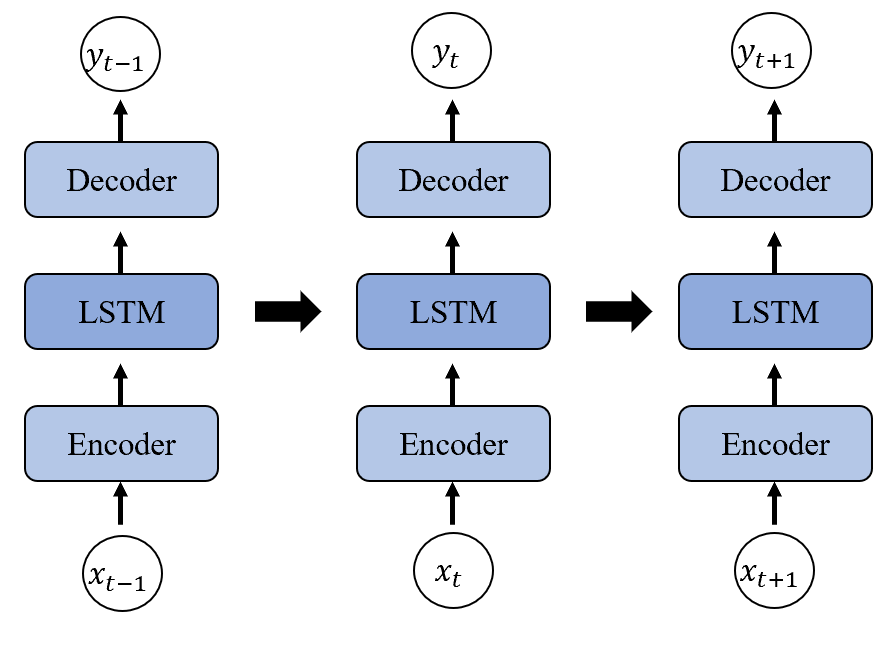
\includegraphics[width=0.6\textwidth]{FigMa/EDR.png}\\
    \vspace{-0.3cm}
    \caption{EDR 网络结构}
    \label{fig:EDR}
\end{figure}
其中$x_t$代表第$t$个时刻的输入的人体姿态,而$y_t$则代表由$x_t$预测出的未来人体姿态。网络接受$x$作为每个RNN节点的输入,首先输入姿态通过编码器(Encoder)编码到隐空间,随后送入RNN层,将时序信息提取并传递给下一个节点。同时通过解码器(Decoder)解码出对应的未来人体姿态作为当前节点的输出。该方法很好地利用了RNN的时序数据建模能力,有效提取了输入人体运动序列中的时序信息。但由于当前RNN节点是在上一个节点的基础上进行预测,因此容易出现误差累积问题。此外,由于在EDR中,未来运动序列被逐时刻、独立地预测,因此在输入序列和预测序列的过渡部分容易出现不连续的现象。
\begin{figure}[ht]
    \centering
    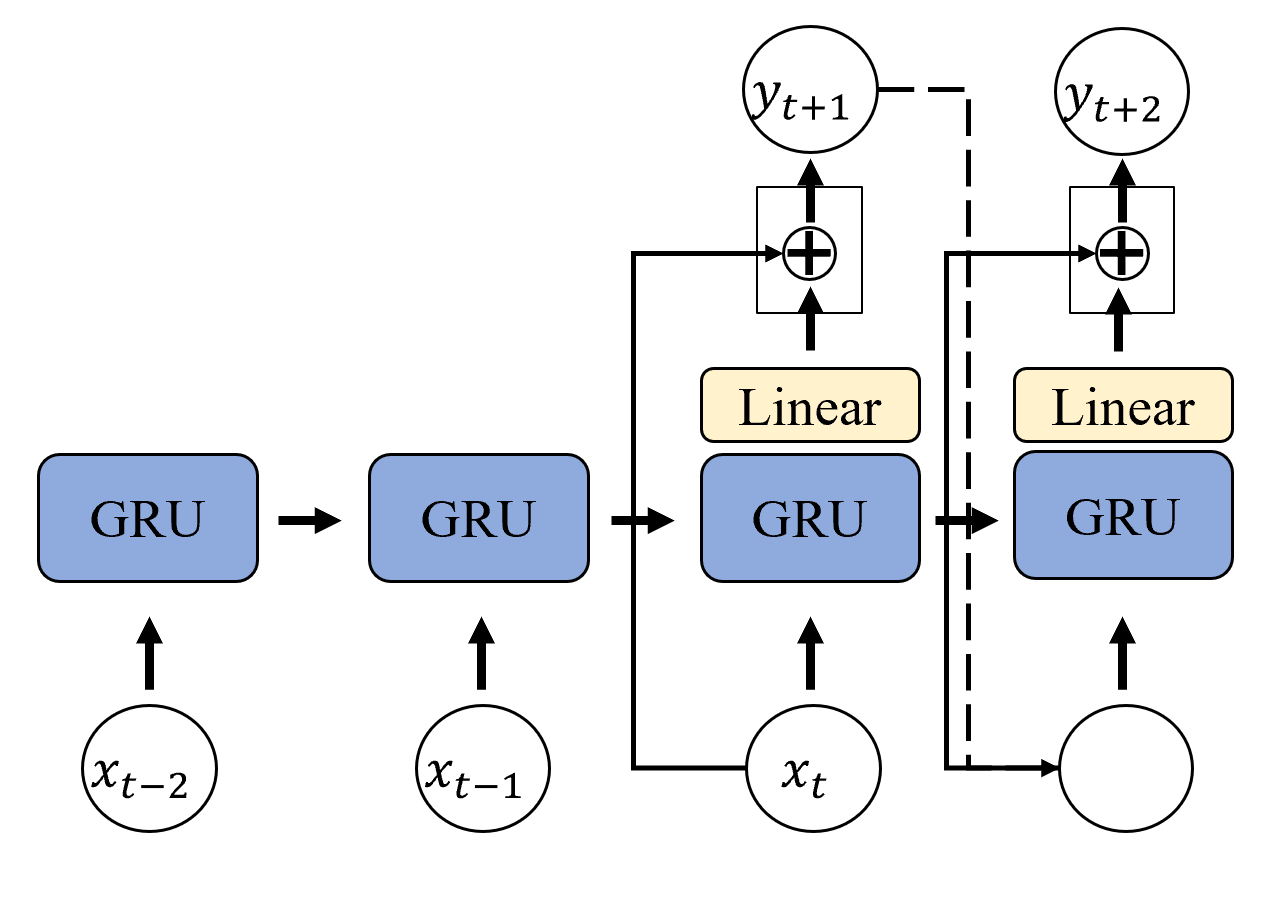
\includegraphics[width=0.6\textwidth]{FigMa/ResSup.png}\\
    \vspace{-0.3cm}
    \caption{Res. Sup. 网络结构}
    \label{fig:ResSup}
\end{figure}
Res. Sup.\parencite{martinez2017human}针对EDR中的问题提出了改进措施,如图\ref{fig:ResSup}所示,Res. Sup.引入了在自然语言处理领域常用的$seq2seq$模型结构,与EDR相比,$seq2seq$统一将输入序列编码到隐空间,此时隐空间包含所有的输入信息,这有助于模型从全局的角度考虑,而不是主要依靠当前时刻的输入。随后通过解码器结构,将隐空间中的信息解码为未来人体运动,当前时刻的输出将作为下一时刻的输入,这有助于保证时序上的连续性,也允许相邻时刻的运动通过残差连接的方式完成一致性约束。除网路结构外,另一些方法从人体运动学入手,通过分析人体运动模式来针对性地设计网络,例如Tang \etal \parencite{tang2018long}发现在人体运动中,并非所有关节点都处于运动状态。相反只有处于肢体末端的关节点位置才会较为频繁地改变。因此,他们提出了针对人体运动模型中频繁运动的关节点的方法,称为HUM。具体的,他们设计了一个新颖的门控单元用来过滤运动幅度小的关节点。此外,注意力机制被用来关注具体的运动模式。AHMR\parencite{liu2022investigating}为了捕获更多的长期相关性,在RNN单元中,可以同时对相邻关节和帧进行编码。此外,它不仅可以同时对本地和全局上下文进行建模,而且还使用了一个注意力模块来帮助更新全局上下文。

虽然上述方法在EDR的基础上提出了改进措施,提升了网络性能,但由于RNN网络的特性任然无法解决诸如误差累积、过渡部分不连续、训练困难和难以处理长时间依赖关系等问题,这将削弱网络预测的真实性。为此一些新的方法的将目光投向了效率更高,感受野更大的卷积神经网络。

\section{基于卷积神经网络}
人体运动序列数据包含时间和空间两个维度,而卷积神经网络(CNN)在处理空间数据上有天然优势,时序信息也可以由1D的CNN(TCN\cite{oord2016wavenet})进行处理,相比循环神经网络,TCN更轻量化、推理速度更快、配合空洞卷积\cite{yu2017dilated}感受野更大。在人体运动预测中,对于模型如何处理空间和时间的依赖关系是一个非常重要的问题。传统的CNNs只能捕捉静态图像的空间依赖性,但是在动态场景下,时间信息也是非常关键的。因此,研究人员提出了一些新的CNN架构,以处理人体运动预测的时空依赖关系。

在Butepage \etal \parencite{butepage2017deep}中,作者设计了一种新的卷积层来编码不同的时间尺度。这种卷积层可以有效地捕捉局部时间尺度的依赖关系,但是它无法处理长期的时间依赖性。为了解决这个问题,QuaterNet\parencite{pavllo2018quaternet}引入了扩张卷积,可以在网络中捕捉长期时间依赖关系。该方法在分层输入姿势的情况下表现良好,但仍然无法处理空间依赖性。

为了同时处理空间和时间的依赖性,一些研究人员采用了分层结构的CNN Li \etal \parencite{li2018convolutional}。这种CNN架构利用卷积结构来捕捉长期隐藏状态,并将其送到解码器中以生成人体姿势。这种方法可以有效地处理时空依赖关系,但是它需要大量的计算资源和训练数据。为了进一步提高模型的性能,Li \etal \parencite{li2019efficient}提出了一种卷积分层自编码器框架,用于表示人体骨骼结构。在这种框架中,分层拓扑被用于表示骨骼结构,并且嵌入了1D卷积层来编码每个节点。该框架可以有效地捕捉空间和时间的依赖关系。
最近,TrajectoryCNN\parencite{liu2020trajectorycnn}被提出来处理人体运动预测的时空依赖关系。它引入了一种新型的轨迹空间,可以轻松地捕捉各种局部-全局和时空特征。这种框架在许多基准测试中取得了优异的性能。

虽然CNN能有效处理时间和空间数据,但CNN的规则卷积核决定它适合处理图像或视频这类规则数据。人体姿态属于不规则的无向图结构,人体关节点对应图中的顶点,骨骼对应顶点间的相互关系。这种拓扑结构是极其重要的先验空间信息,能有效辅助模型感知运动模式。而CNN的规则卷积核使得它很难利用这类先验信息,因此,在最近的研究中,天然具有拓扑信息处理能力的图卷积网络(GCN)获得了越来越多的关注。


\section{基于图卷积网络}
GCN是一种可以处理图形结构数据的神经网络。在GCN中,卷积操作是基于邻居节点之间的连接进行计算的,这使得GCN可以有效地处理具有不规则连接的数据结构,例如人体关键点。此外,GCN还可以利用拓扑信息来捕捉节点之间的关系,从而更好地理解图结构数据。该特性对人体运动序列数据处理非常有利。

%LTD DMGNN ST-GCN 
\begin{figure}[ht]
    \centering
    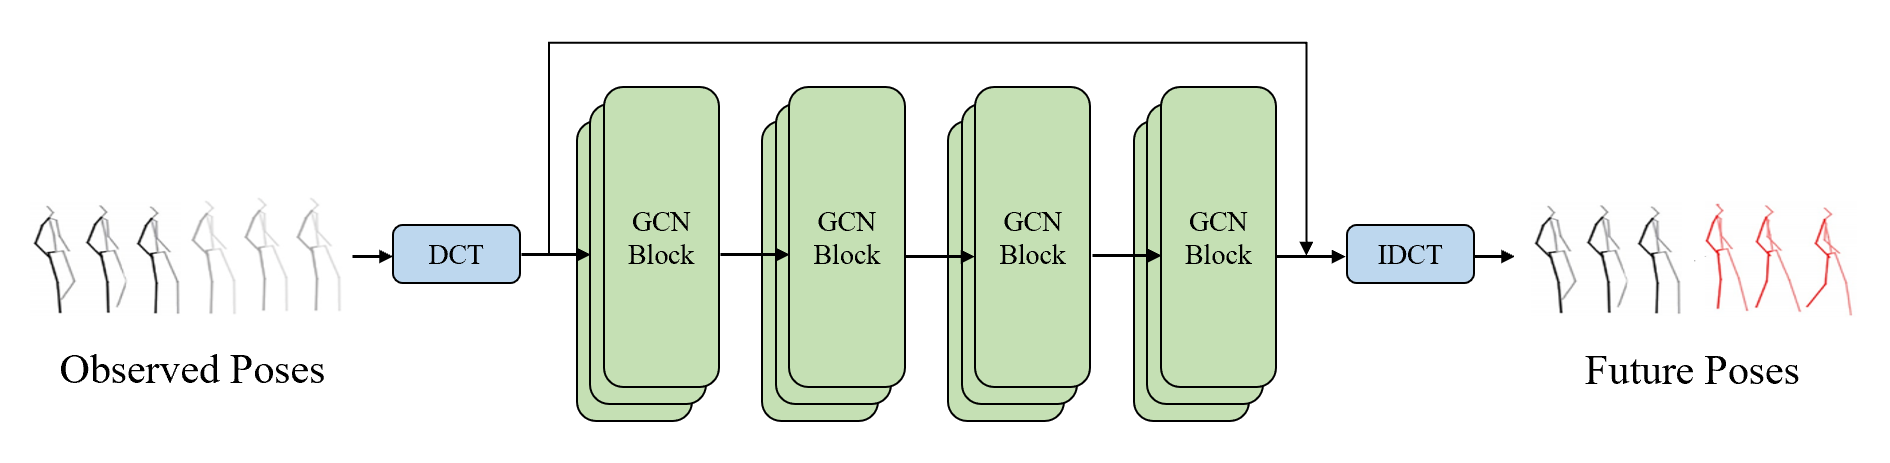
\includegraphics[width=1\textwidth]{FigMa/LTD.png}\\
    \vspace{-0.3cm}
    \caption{LTD 网络结构}
    \label{fig:LTD}
\end{figure}
LTD\parencite{mao2019learning}率先提出了一种代表性的GCN方法(图\ref{fig:LTD}),使用原始的GCN对人体运动序列进行建模。具体的,对于输入的人体运动序列,LTD将其视作一个不规则的无向图。由于人体运动序列数据包含时间和空间两个维度,而原始的GCN只能处理二维平面数据。因此,LTD将该运动序列中的关节点轨迹视作一个整体,将其放入图结构网络中。即图中的每个节点包含了某个关节点这段时间内的运动轨迹,由此LTD实现了使用一个描述平面节点联系的GCN来处理时空维度的人体运动序列。在网络结构方面,网络接受历史人体运动序列作为输入,为了保证输入数据和输出数据在时间维度上的一致性,LTD提出用已知序列的最后一个人体姿态填充输入序列,使其与输出序列时序长度一致。此外,网络输入和输出数据之间的残差连接也得到保证,有助于提高网络的训练效率和预测精确性。完成填充步骤后,输入数据将经过离散余弦变换(DCT)从时域变换到频率域,通过过滤掉低频信息并保留高频信息,可以在降低数据维度的同时,减少噪声。随后,再被传入多个串联的GCN模块,将数据映射到隐空间后,提取时空信息,在填充数据的基础上预测未来运动。最后,经过离散余弦逆变换(IDCT)后,输出最终的预测结果。该方法的贡献在于,提出了一种使用原始GCN对时序数据进行建模的方式,在最终预测精度上大幅领先基于RNN的方法,通过全局的残差连接解决了输入序列和预测序列过渡部分的不连续性。但由于该方法忽略数据的时序特性,仅仅使用GCN提取人体姿态的空间结构信息,将关节点轨迹作为一个整体放入图节点中,这导致该模型对时序运动的感知能力有所欠缺,未来仍然有提升空间。

用于人体姿态提取的方法ST-GCN\parencite{yan2018spatial}针对LTD存在的问题,提出了一种具有时空信息提取能力的GCN。对于时空人体运动序列数据,一个直观的想法是建立一个跨越时空维度的图,囊括不同时间和空间上的关节点。但由于GCN复杂度随着时空维度的增加成倍数上升,这样的图结构数据的复杂度是难以接受的。因此ST-GCN提出将时间和空间维度的数据拆分,分别用TCN\parencite{oord2016wavenet}和GCN进行处理。具体的,1D的卷积神经网络TCN负责提取各个关节点轨迹中的时序数据,GCN负责处理人体姿态中的空间结构数据。通过将时空两个维度分为,ST-GCN将网络的时间复杂度降为线性增长。并且通过实验证明网络时空信息提取能力优于现有方法。但TCN为局部算子,感受野被限制在卷积核范围内,导致ST-GCN在提取长时依赖上存在缺陷。

最近MSR\parencite{dang2021msr},更进一步提出了空间层次化的GCN网络。它提出了一个类Unet\parencite{ronneberger2015u}网络,编码器部分,逐渐简化人体姿态空间结构,只保留最简洁的空间信息。解码器部分,首先构造空间结构较简单的人体运动序列,随着网络的深入,人体运动序列的空间复杂程度逐渐增加,直到输出具有完整空间结构的数据。具体的GCN模块设计上它参考了LTD,将关节点运动轨迹视作一个整体。该方法提出的空间层次化Unet网络,给网络一个渐进式的学习过程,这有利于降低网络的学习难度。但对空间结构进行简化的过程中,破坏了人体结构先验信息,导致网络预测效率相比LTD并没有明显提升,某些方面甚至出现了下滑。

由于GCN网络对图结构数据中节点关系的处理具有先天的优势,因此GCN能够更好地提取人体姿态数据中的结构先验信息。但现阶段的GCN对于时空跨维度信息的处理能力任然有待提高,它们或是忽略某一个维度来降低时间复杂度,或是在信息提取能力和时间效率上做出了妥协。因此,如何平衡模型复杂度和时空信息处理能力,将是未来的一个研究重点。

\section{基于对抗生成网络}
人体运动姿态预测算法的一个主要难点在于,预测过程中存在不确定性,这种不确定性是由于输入序列和预测目标序列之前的差异造成的。例如,如果输入序列与预测目标序列关联性强,则预测越简单,反之则越难。针对上述问题,一个解决思路是如上述方法,通过提高网络的时空信息提取能力,尽可能捕捉输入和预测序列间的关联性。另一个思路是引入生成式模型和随机性,生成更真实的运动序列。具体的,近年来由于对抗生成网络\parencite{goodfellow2020generative}的深入研究,GAN为生成人体运动姿态序列提供了更多新的可能性。

Barsoum \etal \parencite{barsoum2018hp}率先提出了一种基于GAN的$seq2seq$人体运动序列预测方法,它使用改进版的WGAN-GP进行训练,与上述基于RNN,CNN或GCN的方法不同,它的网络输入表达为概率密度分布而非固定的人体运动序列。因此,在预测时可以通过为网络提供不同的随机噪声$z$,来对同一个输入运动序列预测不同的未来运动序列。然而,虽然该方法在结果真实性方面有所提升,但由于输入噪声的引入,预测准确性有所下降。在此基础上,BiHMP-GAN\parencite{kundu2019bihmp}同样通过在输入序列中添加从固定分布中采样的随机噪声来为预测过程添加随机性。不同的是,BiHMP-GAN提出了一个双向对抗神经网络来解决预测过程中的模式坍塌问题。
与此同时,受到上述工作的启发,AGED\parencite{gui2018adversarial}提出了一种新颖的对抗生成框架,它具有两个全局的循环鉴别器,一个鉴别器被用于促进生成序列的保真度,另一个鉴别器与网络进行联合训练,保证未来生成序列的连续性。STMI-GAN\parencite{hernandez2019human}也沿用了该思路,用于处理长时依赖的人体运动序列。Adversarial Refinement Network (ARNet)\parencite{chao2020adversarial}设计了一种新的对抗式的误差调整策略,与上述方法不同的是。判别器不再直接判断生成结果的真实性而是用来估计预测误差,随后精修模块再根据误差调整预测结果。而Lyu \etal \parencite{lyu2021learning}则利用GAN模拟路径积分来解决随机微分方程并预测未来运动轨迹。值得注意的是,由于GAN的对抗训练特性,想要训练达到平衡状态是非常困难的,Cui \etal\parencite{cui2021efficient}提出了一种新的GAN,该GAN使用了spectral归一化,以避免模式坍塌。还有另一种称为AMGAN\parencite{liu2021aggregated}的策略,它由复合GAN结构设计而成,包含用于不同低维身体部位的局部GAN和用于高维全身的全局GAN组成。该方法证明了降维可以有效地提高GAN的训练效率。

总而言之,利用GAN的策略主要可分为两类。(1) 被用作学习算法以帮助网络生成更加真实的结果。(2) 利用随机噪声向网络添加随机性,生成多样化的预测结果。而GAN作为一个具有明显优势和劣势的网络,也会给研究人员的工作带来一定的挑战。
\section{基于Transformer}
近些年,Transformer受到了学术界的广泛关注,它也从自然语言处理(NLP)领域被引入到计算机视觉领域,在诸如图片识别、图片分割等经典问题上大幅领先现有基于卷积神经网络的方法。对于人体运动序列预测问题,网络需要捕捉长时依赖关系的能力。而Transformer的全局感受野特点恰好可以解决该问题。因此出现了一批基于Transformer的方法\parencite{aksan2021spatio, cai2020learning}。

Aksan \etal \parencite{aksan2021spatio}设计了一个包含时间和空间分支的Transformer网络,两个分支分别提取输入序列的空间结构信息和时序信息,最后再通过融合模块得到最后的预测结果。

\begin{figure}[ht]
    \centering
    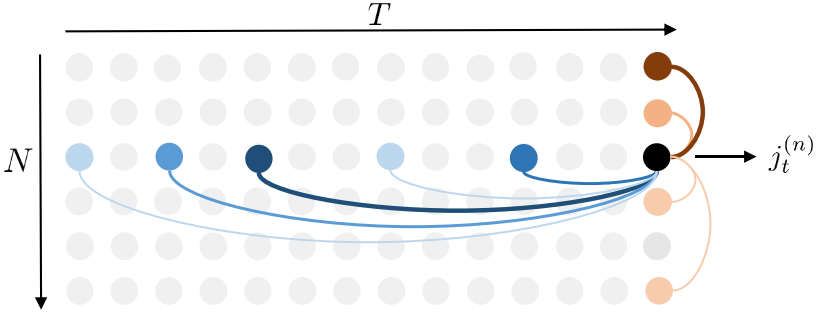
\includegraphics[width=0.8\textwidth]{FigMa/ST-Transformer.png}\\
    \vspace{-0.3cm}
    \caption{Spatial-temporal Transformer\cite{aksan2021spatio}}
    \label{fig:Spatial-temporal_Transformer}
\end{figure}

其中spatial-temporal Transformer原理如图\ref{fig:Spatial-temporal_Transformer}所示,$j^{(n)}_t$表示$t$时刻,第$n$个关节点。其中,$j^{(n)}_t$只和自己位于同一时间或空间的关节点进行注意力(attention)机制计算,图中颜色的深浅代表关节点之间的关联程度,颜色越深关联性越强,权值也越高,反之则越小。通过分离的时空transformer,该方法间接地提取了时间和空间信息。

\begin{figure}[ht]
    \centering
    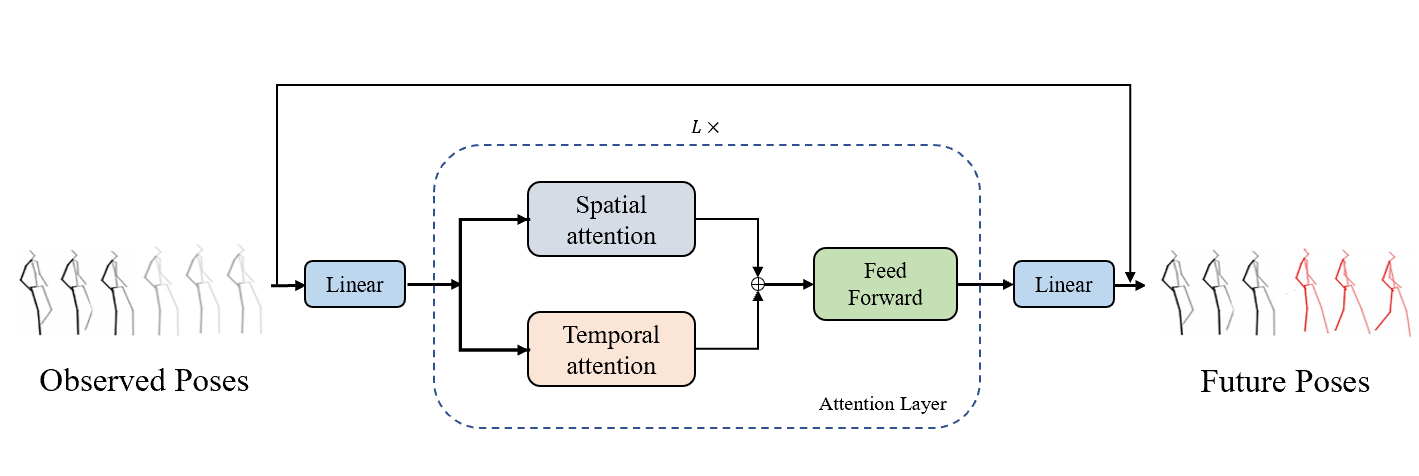
\includegraphics[width=1\textwidth]{FigMa/ST_Transformer.png}\\
    \vspace{-0.3cm}
    \caption{Spatial-temporal Transformer\cite{aksan2021spatio}}
    \label{fig:Spatial-temporal_Transformer网络结构}
\end{figure}

完整的网络结构如上图所示,网络由$L$个串联的注意力层构成,每个层包含一个空间维度和时间维度的注意力层,特征被传入注意力层后,分别送往两个分支,用于提取时间和空间信息。提取结束后,空间和时间信息相加,送入前馈神经网络进行特征融合,最终通过线性层输出预测的未来人体运动序列。该方法通过并行的方式分离时间和空间维度,减少了时间复杂度和模型参数量。但分支的方法使得时间和空间维度缺少信息通信手段,导致信息交流受阻,影响最终的模型质量。总的来说,Transformer高效的全局注意力机制有利于模型捕捉长时序依赖,但Transformer的注意力计算模块也导致模型空间的上升和计算开销的增加。此外,时间和空间分支间的通信问题也是未来需要研究的问题。

%看情况还写不写另一个方法的介绍。

\section{总结}
本章,我们对人体运动姿态预测算法的发展做了一个简要的回顾。在初期,研究人员根据循环神经网络在处理时序数据上的优势,设计了$seq2seq$的网络模型来对输入序列统一编码后预测未来运动序列。但由于循环神经网络对于时序记忆的能力依赖隐变量的大小,因此难以处理长时依赖。此外,梯度消失等训练问题也困扰着现有方法。随后,研究人员将目光转向了卷积神经网络,特别是图卷积神经网络,它对无结构不规则数据的处理有天然的优势。但如何对传统图卷积网络进行改进,使其拥有时序信息处理能力,任然是当前的研究热点。此外,GAN机制的引入允许生成更多样化和真实的结果,但其训练过程的不稳定性和噪声对结果准确性的影响有待进一步解决。近些年,Transformer的兴起给该问题带来了新的解决思路,其全局感受野的特性,允许其捕捉更长范围的全局依赖。但其注意力计算带来的额外计算开销和时空信息间的通信问题,还需要进一步探索。本文希望在现有基于图卷积的方法的基础上,提高模型的时空信息提取能力,并且控制模型的运行开销。



	\chapter{图卷积网络基础}
\section{图卷积网络简介}
图卷积网络(Graph Convolutional Networks,GCN)是一种用于图像数据处理的神经网络模型。与传统的卷积神经网络(Convolutional Neural Networks,CNN)不同,GCN能够处理图像结构数据,并且能够通过学习节点之间的关系来推断节点的特征。GCN的发展是为了解决传统CNN在处理非欧几里德结构的数据时,面临的局限性和挑战性。

GCN的应用广泛,包括社交网络分析、推荐系统、化学和生物信息学等领域。例如,GCN可以用于社交网络中的节点分类任务,其中每个节点代表一个用户,而用户之间的关系可以通过社交网络的拓扑结构表示。通过学习这些节点之间的关系,GCN可以有效地预测新用户的属性,例如他们的兴趣爱好或职业等。

GCN的核心思想是利用卷积操作来对节点进行特征提取。由于图像数据的非欧几里德性质,传统的卷积操作无法直接应用于图像数据。因此,GCN引入了一种局部聚合的方式来计算每个节点的特征。具体来说,GCN利用节点的邻居信息来计算该节点的新特征,并通过非线性变换来实现特征提取。

GCN的结构可以看作是一个多层感知机(Multilayer Perceptron,MLP),其中每一层对邻居节点进行聚合,并通过激活函数进行非线性转换。每一层的输出都可以被视为该节点的新特征,这些新特征又被用于下一层的聚合。在图像分类和节点分类任务中,GCN通常通过全局平均池化来获得最终的输出。

最近,许多新的GCN变体已经被提出,例如Graph Attention Network(GAT)、GraphSAGE、ChebNet等等。这些变体使用不同的方法来聚合节点的邻居,并具有更好的性能和可扩展性。例如,GAT利用注意力机制来计算不同节点之间的权重,可以更加灵活地处理节点之间的关系。

总之,GCN是一种强大的图像处理方法,它可以有效地学习节点之间的关系,并利用这些关系来推断节点的特征。它已经被广泛应用于各种领域,成为了图像处理领域的重要工具。GCN的发展也为处理非欧几里德结构的数据提供了新的思路和方法。

\section{图卷积模型定义} \label{gcn_model_define}
\begin{figure}[ht]
    \centering
    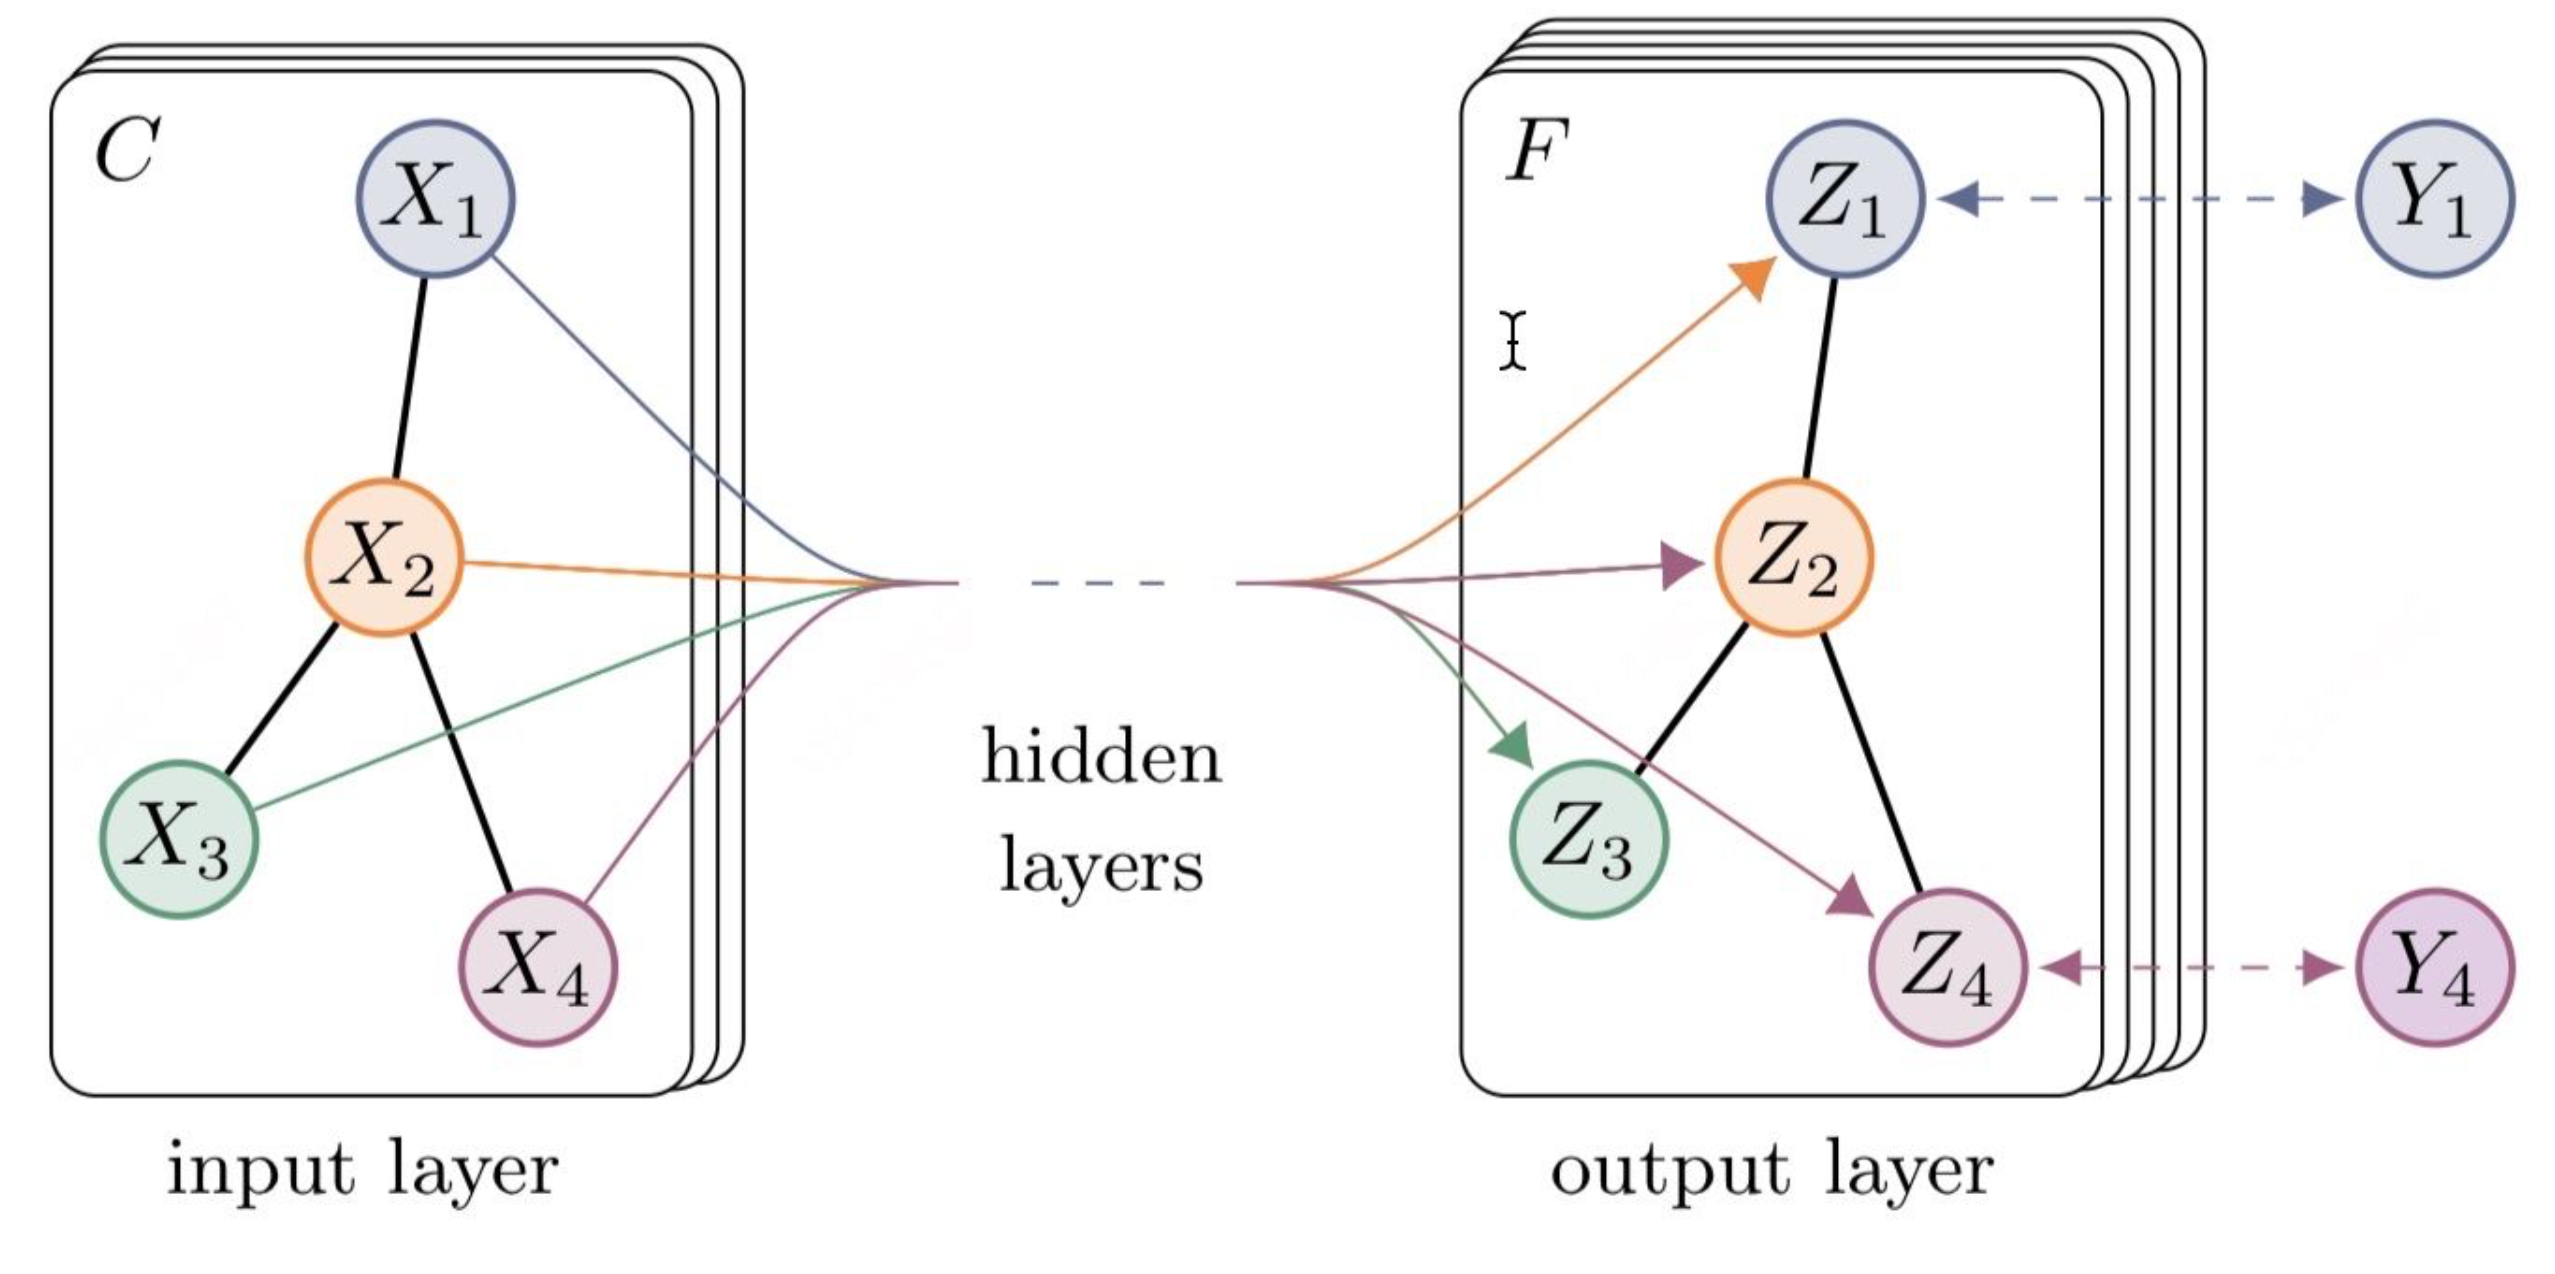
\includegraphics[width=0.80\textwidth]{FigMa/GCN-SEMI.png}\\
    \vspace{-0.3cm}
    \caption{图卷积示意图,来自\parencite{kipf2016semi}}
    \label{fig:GCN-SEMI}
\end{figure}
图\ref{fig:GCN-SEMI}展示了一个标准的GCN。可以看到一个具有个$C$个输入通道的图结构数据通过中间的隐藏层,产生了$D$个通道的输出。在这一过程中,GCN不改变图的空间结构,只是对节点特征进行变换,参考图中各节点的信息流动趋势,捕捉空间结构信息。本文将网络的输入$X$定义为一个$V*D$的矩阵,其中$V$代表输入图中的节点数量,而$D$代表输入图中节点的特征维度。$X$经过特征处理后即可得到输出$Z$,一个维度为$V*D^{\prime}$的矩阵,其中$V$结构不变,$D^{\prime}$为变换后的特征维度。

一个图的空间结构可以用邻接矩阵描述。邻接矩阵是一种用于表示图形或网络的数据结构。它是一个方阵,其中行和列分别对应于图中的节点,矩阵中的每个元素表示两个节点之间是否存在一条边。具体来说,假设图有$V$个节点,那么邻接矩阵的大小为$V \times V$。如果节点$i$和节点$j$之间存在一条边,则邻接矩阵中第$i$行第$j$列的元素为1;如果它们之间不存在边,则该元素为0。邻接矩阵还可以用于表示带权图,其中矩阵中的元素表示边的权重。如果节点$i$和节点$j$之间存在一条权重为$w$的边,则邻接矩阵中第i行第j列的元素为$w$;如果它们之间不存在边,则该元素为0或一个特殊的表示不存在边的值(如-1)。邻接矩阵是一种简单且直观的图表示方法,适用于图比较稠密(边数接近节点数的平方)的情况。但是,对于稀疏图(边数远小于节点数的平方)来说,邻接矩阵会浪费大量的空间。此时,邻接矩阵的时间和空间复杂度可能较高,因此在应用时需要针对稀疏矩阵进行额外的优化。在定义邻接矩阵以后,可以很轻易重构一个图结构。本文用$G=(V,E)$定义一个图,其中$V$代表节点,$E$代表边。通过$\left|V\right| \times \left|V\right|$得到$A$,其中如果节点$i$和节点$j$之间存在联系,则$A_{ij}=1$否则则等于0。由此,便通过一个图数据结构结构得到邻接矩阵$A$,同理也可以根据$A$得到一个图数据结构。
\begin{figure}[ht]
    \centering
    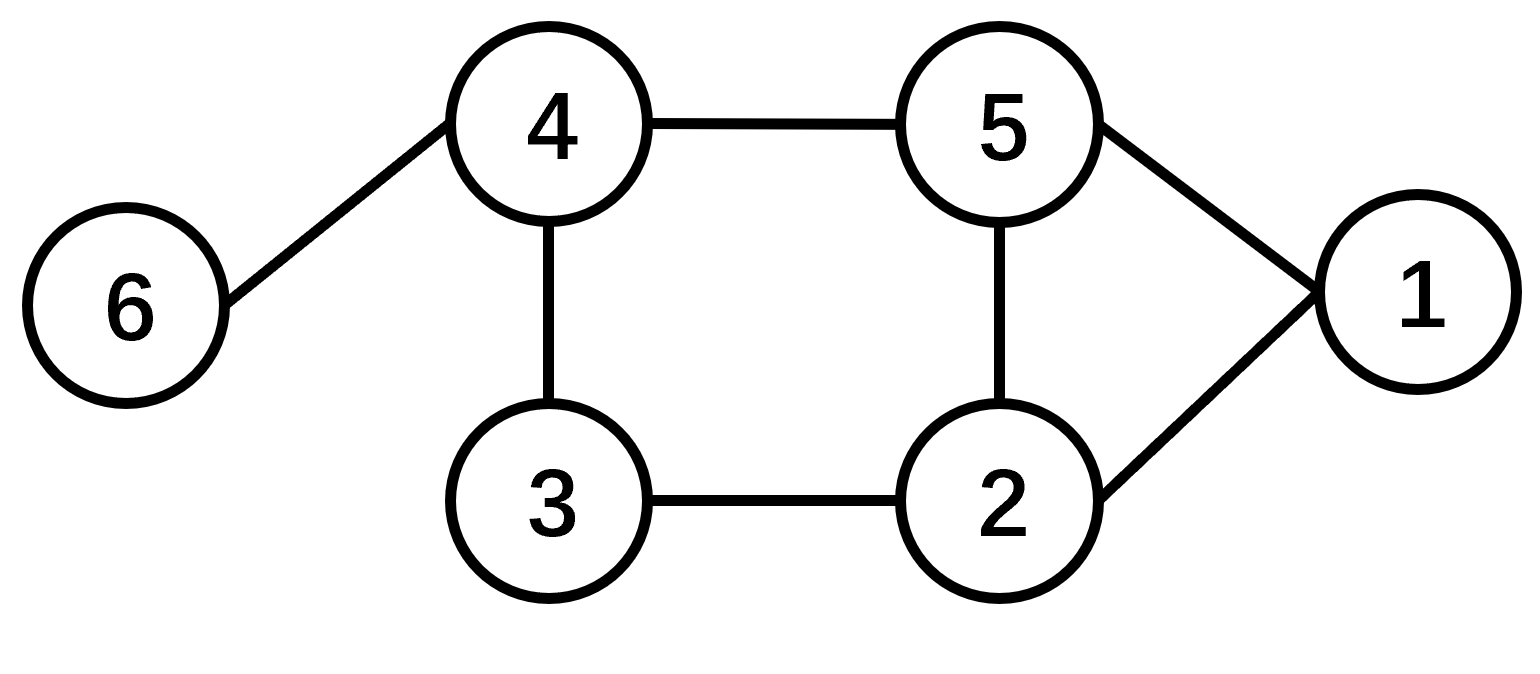
\includegraphics[width=0.70\textwidth]{FigMa/Graph_structure.png}\\
    \vspace{-0.3cm}
    \caption{图结构数据示意图}
    \label{fig:Graph_structure}
\end{figure}
如上图所示,本文定义了一个拥有6个节点的图结构数据。其中节点上的数字代表该节点的编号,节点间的连接代表两点间存在联系。根据上文,可以将该图的数据结构以邻接矩阵的形式表示如下。
\begin{equation}
\begin{pmatrix}
        0 & 1 & 0 & 0 & 1 & 0 \\
        1 & 0 & 1 & 0 & 1 & 0 \\
        0 & 1 & 0 & 1 & 0 & 0 \\
        0 & 0 & 1 & 0 & 1 & 1 \\
        1 & 1 & 0 & 1 & 0 & 0 \\
        0 & 0 & 0 & 1 & 0 & 0 \\
\end{pmatrix}
\label{equation:adj_mat}
\end{equation}
其中有联系的关节点则被置为1。例如,由于1号节点和5号节点之间存在连接,则$A_{15}$和$A_{51}$均被置为1且因为图\ref{fig:Graph_structure}为无向无环图,因此邻接矩阵沿着对角线对称,对角线上的元素均为0。所以可以根据邻接矩阵将图卷积网络中的一层定义为如下非线性函数:
\begin{equation}
   H^{(l+1)} = f(H^{(l)} ,A)
    \label{equation:GCN_simple_define}
\end{equation}
其中$H$为该层的隐变量,其中输入层$H(0)=X$,输出层$H(L)=Z$,L代表最后一层,$Z$为最终输出网络的结果。不同的GCN函数,使用不同的GCN模型$f(\cdot,\cdot)$。被广泛传播的图卷积层定义如下:
\begin{equation}
    f(H^{(l)},A) = \sigma\left( \hat{D}^{-\frac{1}{2}} \hat{A} \hat{D}^{-\frac{1}{2}} H^{(l)}W^{(l)} \right)
    \label{equation:GCN_define}
 \end{equation}
其中$D$代表图结构的度矩阵,$W$为每一个卷积层的权重,该公式的物理含义为,当前层隐变量是由上一层隐变量以邻接矩阵为权重加权求和后,再经过线性变换$W$和激活函数得到的。

为了方便理解,本文先定义一个简单的函数$f(H^{(l)},A)$为基础,逐渐推导得到公式\ref{equation:GCN_define}。本文首先定义一个简单的图卷积层级传导公式:
\begin{equation}
    f(H^{(l)},A) = \sigma\left( {A}H^{(l)}W^{(l)} \right)
    \label{equation:GCN_define_base}
 \end{equation}
 在公式\ref{equation:GCN_define_base}中本文通过$A$和$H$矩阵相乘的形式完成简单的加权求和计算。然后在由权重矩阵$W$对节点特征维度进行变换,最后通过激活层$\sigma$得到该层的特征矩阵。$AH$的直观理解是,将于自身相邻的节点特征(信息)加权求和后得到更新后的特征。

 但在这一过程中,更新后的特征只包含周围节点的信息,不包括自身的原始信息(因为邻接矩阵中对角线元素为0,即图中不存在自身回环。)。为此,可以另$\hat{A} = A + I$向邻接矩阵中手动添加自身回环。其中$I$为单位矩阵。此外,如果要进行加权求和,则必须保证权值和为1,否则特征数值会迅速膨胀。因此还需要对$\hat{A}$进行归一化。本文对$\hat{A}$中每一行除以该行的和,即该节点的度。于是$\hat{A}$被归一化为$\hat{D}^{-1}\hat{A}$,在实际操作中通常使用对称归一化,于是便得到了公式\ref{equation:GCN_define}中的邻接矩阵$\hat{D}^{-\frac{1}{2}}\hat{A}\hat{D}^{-\frac{1}{2}}$。代入公式\ref{equation:GCN_define_base}即可得到图卷积公式\ref{equation:GCN_define}。在理解图卷积的直观意义和公式由来后。接下来,本文将借助拉普拉斯算子给出公式\ref{equation:GCN_define}的推导过程以及数学含义,从数学的角度解释图卷积网络的设计逻辑。
\section{拉普拉斯算子}
为了推导图卷积网络,本文将首先介绍拉普拉算子(Laplace operator)作为铺垫,进而给出图卷积网络的数学定义。拉普拉斯算子被定义为欧几里得空间中,一个二阶可微函数$f$梯度的散度,即对该函数求二阶微分,结果表示为$\Delta f$其中$\Delta$代表拉普拉斯算子。如果$f$是图上定义的一组高维向量,则$Lf$是在图空间求二阶微分,其中$L$为拉普拉斯矩阵。为了叙述方便,本文首先在连续欧式空间中,定义$f(x,y,z)$为一个二阶可微的三元函数,在该函数上分别对梯度和散度进行定义。

\subsection{连续空间中的拉普拉斯算子}
梯度是一个矢量,表示某一函数在沿着该点的方向导数上可以取得局部极值。即函数在该方向上沿着该方向下降速度最快,变化率最大。对于位于欧式空间中,一阶可微的函数$f(x,y,z)$。在该函数上一点$P(x,y,z)$,称向量:
\begin{equation}
    \left\{ \frac{\partial f}{\partial x}, \frac{\partial f}{\partial y}, \frac{\partial f}{\partial z} \right\}= \frac{\partial f}{\partial x}\vec{i} + \frac{\partial f}{\partial y}\vec{j} + \frac{\partial f}{\partial z}\vec{k}
    \label{equation:grad}
\end{equation}
为$f(x,y,z)$在点$P$处的梯度,记为$gradf(x,y,z)$或$\nabla f(x,y,z)$,其中$\nabla = \frac{\partial}{\partial x}\vec{i} + \frac{\partial}{\partial y}\vec{j} + \frac{\partial}{\partial z}\vec{k}$。

散度($\nabla \cdot$ )被定义为空间中各矢量场的发散程度,某点的散度被定义为$div(F)$,散度大于零的点代表该点向周围散播能量,而散度小于零的点代表该点向周围吸收能量。当某点散度为0时,则代表该点即不发散也不吸收能量,为无源点。

在了解散度和梯度在连续函数空间中的定义后,即可给出连续二阶可微函数空间中,拉普拉斯算子的具体定义。对于三维函数$f(x,y,z)$,拉普拉斯算子被定义为梯度($\nabla f$)的散度($\nabla \cdot$)。$\Delta f = \nabla^2 f = \nabla \cdot \nabla f = div(grad f)$,在笛卡尔坐标系下被表示为公式\ref{equation:laplace_operator}$(a)$,从三维拓展到在$n$维空间后,拉普拉斯算子被表示为公式\ref{equation:laplace_operator}$(b)$:
\begin{equation}
    \begin{aligned}
        \Delta f &= \frac{\partial^2 f}{\partial x^2}, \frac{\partial^2 f}{\partial y^2}, \frac{\partial^2 f}{\partial z^2} (a)
        \\
        \Delta &= \sum_{i=1}^{n} \frac{\partial^2}{\partial x^2_i} (b)
   \end{aligned}
    \label{equation:laplace_operator}
\end{equation}

\subsection{离散空间中的拉普拉斯算子}\label{discrate_laplace}
在公式\ref{equation:laplace_operator},本文给出了在连续二阶可微函数上的拉普拉斯算子定义。然而,图卷积网络所处理的图结构数据位于离散空间中,需要进一步给出离散空间中的拉普拉斯算子。本文首先从一维离散空间中进行推导。对于位于一维离散空间中的函数$f(x)$,设离散函数空间中的最小间隔为$h$,则$f(x)$在$x_i$处的一阶微分为:

\begin{equation}
    f(x_i)^{\prime} = \frac{ f(x_{i+1}) - f(x_{i+1}) }{2h} 
    \label{equation:frist_order}
\end{equation}

使用同样的方法计算$f(x)$在$x_i$处的二阶微分,可得:
\begin{equation}
    f(x_i)^{\prime \prime} = \frac{ f(x_{i+1}) + f(x_{i+1}) - 2f(x_i) }{h^2} 
    \label{equation:second_order}
\end{equation}

在一维基础上进行推广,可以获得拉普拉斯算子在离散二维空间上的表达式,公式\ref{equation:2d_laplace}展示了离散二维空间中的函数$f(x,y)$的拉普拉斯算子表达式。

\begin{equation}
    \begin{aligned}
        \Delta f &= \frac{\partial^2 f}{\partial x^2} + \frac{\partial^2 f}{\partial y^2} \\
        &= f(x+1, y) + f(x-1, y) - 2f(x, y) + \\
        &\ f(x, y+1) + f(x, y-1) + 2f(x, y) \\
        &= f(x+1, y) + f(x-1, y) + \\
        &\ f(x, y+1) + f(x, y-1) - 4f(x,y)
    \end{aligned}
    \label{equation:2d_laplace}
\end{equation}

由公式\ref{equation:2d_laplace}可以直观的看到,对于离散二维空间中的点$(i,j)$, 该点的拉普拉斯算子值由该点和四个方向上的相邻点的特征值之差得到。这代表拉普拉斯算子可以描述相邻离散点之间的信息差异,反应了信息的流动趋势。当$\Delta f > 0$表示该点的信息将会流向相邻节点,当$\Delta f < 0$时,四周节点的信息流向该节点,当$\Delta f = 0$时,则关节点间不发生信息流动。由于拉普拉斯算子可以很好的描述离散节点间的信息流动方向和强度。因此,在图卷积网络中被用来描述相邻关节点间的信息流动趋势,具体方式本文将在下一章详细叙述如何使用拉普拉普算子推导图卷积网络公式。当前,本文首先给出图结构数据下的拉普拉斯算子定义。

对具有$V$个节点的图$G$,本文将其定义为一个$V$维的向量$G=(x_1, \cdots, x_V, E)$,$x_i$表示第$i$个节点的特征值,$E$为边的集合,通过公式\ref{equation:2d_laplace}将图结构数据中的拉普拉斯算子定义为:
\begin{equation}
    \begin{aligned}
        \Delta x_i &= \sum_{j \in V}A_{ij}(x_i - x_j) \\
        &=\sum_{j \in V}A_{ij}x_i - \sum_{j \in V}A_{ij}x_j \\
        &= d_i x_i - A_{i:}H
    \end{aligned}
    \label{equation:nd_laplace}
\end{equation}
其中$d_i$是节点$x_i$的度。$A_{i:} = (A_{i1},\cdots, A_{iV})$, $H = (x_1, \cdots, x_V)^T$,$A_{i:}H$为这两个向量的内积。

公式\ref{equation:nd_laplace}仅仅给出了单个节点拉普拉斯算子的计算方法,本文将其推广到图中的所有节点,以矩阵形式表示拉普拉斯算子,该矩阵则被称为拉普拉斯矩阵。
\begin{equation}
    \begin{aligned}
        \Delta G &= \left(  \begin{array}{cccc}
            \Delta x_1 \\
            \vdots \\
            \Delta x_V
         \end{array} \right) = 
         \left(  \begin{array}{cccc}
            d_1x_1 - A_{1:}H \\
            \vdots \\
            d_Vx_V - A_{V:}H
         \end{array} \right)
        \\
        & =diag(d_i)H - AH \\
        & = (D-A)H \\
        & = L(G)
    \end{aligned}
    \label{equation:nd_laplace_mat}
\end{equation}

公式\ref{equation:nd_laplace_mat}给出了图结构数据中的拉普拉斯矩阵$L(G)$。其中$D$为度矩阵,$A$为邻接矩阵,它将作为图卷积网络中的重要组成部分。

\section{图卷积网络推导}
在\ref{discrate_laplace}节中,本文得到了图结构数据$G$的拉普拉斯矩阵$L(G) = (D-A)H$,对该拉普拉斯矩阵进行对称归一化后可得:
\begin{equation}
    \begin{aligned}
        L^{norm} &= D^{-\frac{1}{2}}L D^{-\frac{1}{2}} \\
        &= D^{-\frac{1}{2}}(D-A)D^{-\frac{1}{2}} \\
        &= I - D^{-\frac{1}{2}}A D^{-\frac{1}{2}}
    \end{aligned}
    \label{equation:norm_laplace}
\end{equation}
该归一化矩阵,对角线为1,非对角线为$-\frac{1}{\sqrt{deg(x_i)deg(x_j)} }$。

本文希望通过傅里叶级数处理图卷积过程,可两个函数的卷积定义如下:
\begin{equation}
    f*g = \mathcal{F}^{-1}\{\mathcal{F}\{f\} \cdot \mathcal{F} \{ g \} \}
    \label{equation:f_convolution}
\end{equation}
其中$\mathcal{F}$为傅里叶级数。假设$L(G)$的特征值为$\Lambda$,特征向量为$U$。在图卷积网络中,傅里叶变换对应$\mathcal{G}\mathcal{F}\{x\} = U^Tx$,对应的其逆变换为$\mathcal{I}\mathcal{G}\mathcal{F}\{x\} = Ux$,将二者代入公式\ref{equation:f_convolution}中即可得到对应的图卷积公式。
\begin{equation}
    \begin{aligned}
        g * x &= \mathcal{I}\mathcal{G}\mathcal{F}\{ \mathcal{G}\mathcal{F}\{g\} \cdot \mathcal{G}\mathcal{F}\{x\} \} \\
        &=U(U^Tg \cdot U^Tx) 
    \end{aligned}
    \label{equation:gcn_f}
\end{equation}
本文将$g$定义为一个以拉普拉斯矩阵为参数的函数$g(L)$,其作用是传播或接受周围邻居的信息。因为有$U^T L = U^T U \Lambda U^T = \Lambda U^T$,所以本文进一步将$U^T g$看作是以拉普拉斯矩阵特征值为参数的函数$g_\theta(\Lambda) = diag(\theta)$,其中$\theta$为参数。随后,在频率域上,公式\ref{equation:gcn_f}可以简化表示为:
\begin{equation}
    g_\theta x= Ug_\theta U^T x
    \label{equation:gcn_f_2}
\end{equation}

为了简化计算,本文采用$Chebyshev \ polynomials$将$g_\theta$近似为:
\begin{equation}
    g_{\theta^{\prime}} * x \approx \sum_{k=0}^{K} \theta^{\prime}_k T_k (\widetilde{\Lambda})  
    \label{equation:g_approx}
\end{equation}

其中$\widetilde{\Lambda} = \Lambda - I$,$K$表示经过了$K$阶拉普拉斯矩阵的处理。$T_k(x) = 2xT_{k-1}(x) - T_{k-2}(x)$,同时$T_0 = 1$,$T_1 = x$。上述近似计算代入公式\ref{equation:gcn_f_2}可得:

\begin{equation}
    \begin{aligned}
        g_\theta x &= Ug_\theta U^T x \\
        &\approx U \sum_{k=0}^{K} \theta^{\prime}_k T_k (\widetilde{\Lambda}) U^Tx
        &=\sum_{k=0}^{K} \theta^{\prime}_k T_k (U\widetilde{\Lambda}U^T)x
        &=\sum_{K}^{k=0} \theta^{\prime}_k T_k(\widetilde{L})x
    \end{aligned}
    \label{equation:gcn_3}
\end{equation}
其中$\widetilde{L} = L - I$,由于一个GCN只包含一次信息传递过程,只拥有一个一阶的拉普拉斯矩阵,因此取$k=1$代入公式\ref{equation:gcn_3},可得到如下所示的图卷积计算公式:
\begin{equation}
    \begin{aligned}
        g_\theta x &=\sum_{1}^{k=0} \theta^{\prime}_k T_k(\widetilde{L})x \\
        &=\theta^{\prime}_0 T_0(L-I)x + \theta^{\prime}_1 T_1(L-I)x \\ 
        &=\theta^{\prime}_0x + \theta^{\prime}_1(L-I)x\\
        &=\theta^{\prime}_0x + \theta^{\prime}_1(I-D^{-\frac{1}{2}}AD^{-\frac{1}{2}}-I)x\\
        &=\theta^{\prime}_0x - \theta^{\prime}_1 D^{-\frac{1}{2}}AD^{-\frac{1}{2}} x
    \end{aligned}
    \label{equation:gcn_4}
\end{equation}

为了减少参数和降低模型复杂度,设$\theta = \theta^{\prime}_0 = -\theta^{\prime}_1$,同时令$\hat{A} = I+A$和$\hat{D}_ii = \sum_{j \in V}\hat{A}_ij$,可得:
\begin{equation}
        g_\theta * x =\theta \hat{D}^{-\frac{1}{2}}\hat{A} \hat{D}^{-\frac{1}{2}} x
    \label{equation:gcn_5}
\end{equation}

再加上激活函数$\sigma$,即可得到\ref{gcn_model_define}节中提到的图卷积模型计算公式:
\begin{equation}
    f(H^{(l)},A) = \sigma\left( \hat{D}^{-\frac{1}{2}} \hat{A} \hat{D}^{-\frac{1}{2}} H^{(l)}W^{(l)} \right)
    \label{equation:GCN_define_2}
 \end{equation}

其中$H$为输入的特征向量,$W$代表参数$\theta$。在实际使用中,为了降低模型的复杂度,通常将$A$定义为可学习的参数矩阵,由网络进行归一化,因此模型被简化为:

\begin{equation}
    f(H^{(l)},A) = \sigma\left(\hat{A}H^{(l)}W^{(l)} \right)
\end{equation}


\subsection{总结}
在本章节中,本文介绍了图卷积的基本概念,包括图结构、拉普拉斯算子、谱理论和特征表示等。拉普拉斯算子是图卷积的核心概念之一,通过计算它可以得到图的特征表示。接着,本文又推导了图卷积公式,介绍了如何使用卷积神经网络在图上进行卷积操作,进一步拓展了图卷积的应用。

首先,图卷积是一种用于处理图数据的卷积操作,可以用于学习图的结构信息。其次,拉普拉斯算子是计算图卷积的核心算子之一,它可以将图的结构信息转化为数学表达形式,为图卷积提供了理论基础。第三,谱理论是图卷积的重要理论基础之一,通过它可以了解拉普拉斯算子的性质和作用。最后,特征表示是图卷积的重要应用之一,它可以将图的信息转化为向量表示,方便进行机器学习任务的处理。

在对基本的图卷积网络知识进行一定的一定的铺垫后,在后续的内容中,本文将详细介绍提出的基于渐进式策略的人体运动姿态预测算法,主要包含训练策略和网络结构设计两部分
。
% 参考文章
% https://zhuanlan.zhihu.com/p/85287578
% https://zhuanlan.zhihu.com/p/107162772
	\chapter{基于渐进式策略的多阶段人体运动姿态预测框架}\label{chapter-5}
本章节将围绕本文的一个主要贡献点——基于渐进式策略的多阶段人体运动姿态预测框架进行介绍。分别从动机、方案、实现和算法细节几个方面对本方法进行详细的阐述。在此之前,本文首先通过数学语言定义人体运动姿态预测问题,并介绍在此过程中使用的相关数据结构,以方便在本文后续章节中进行准确的叙述。
\section{人体运动姿态预测问题的数据描述与问题定义}
\subsection{人体运动姿态数据结构}
\begin{figure}[ht]
    \centering
    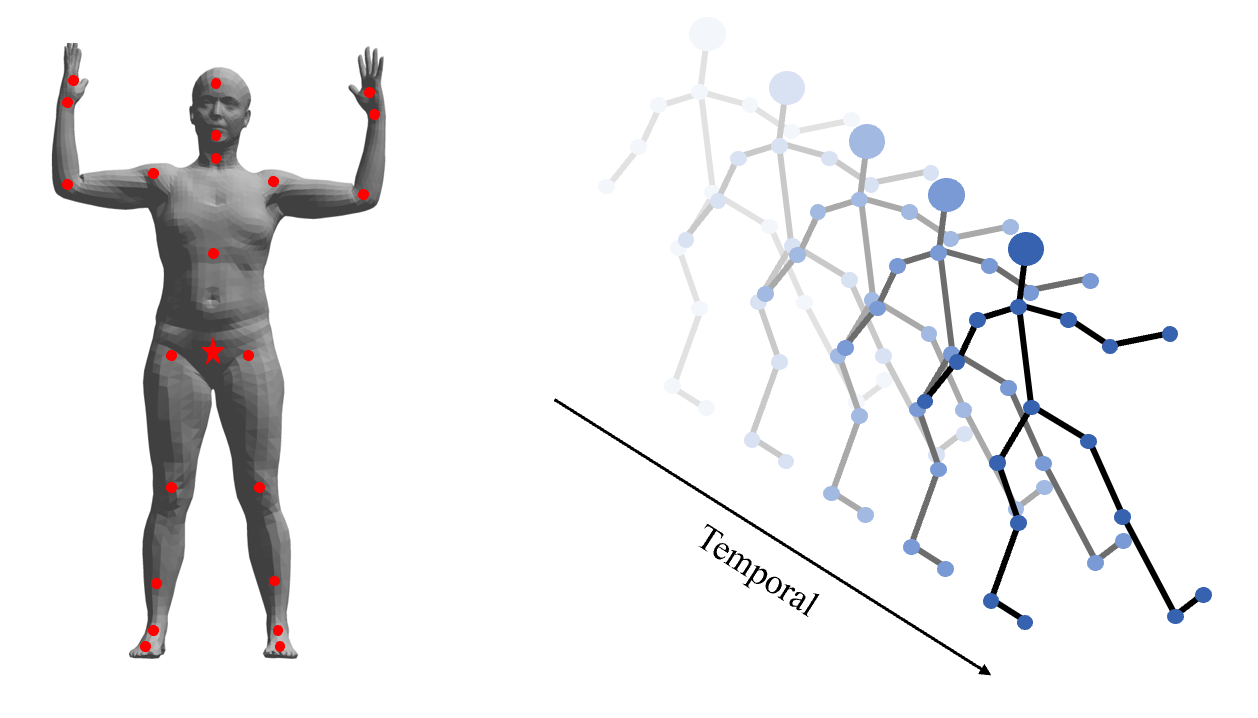
\includegraphics[width=0.85\textwidth]{FigMa/show_structure.png}\\
    \vspace{-0.3cm}
    \caption{人体运动姿态数据结构}
    \label{fig:data_structure}
\end{figure}
首先本文介绍人体运动姿态预测问题所使用的数据结构。如图\ref{fig:data_structure}左所示,人体运动数据是通过动作捕捉设备,在封闭室内或开放室外场景中提取到的人体关键点运动序列,这些数据以SKT(Skeletal Kinematic Tree)的形式表示和存储。在实际动作捕捉过程中,通常只关注在运动过程中起决定性作用的关节点,例如手肘、肩部、膝盖等。这些关节点在图\ref{fig:data_structure}左中以红色标记的形式展现。其中位于胯部的五角星节点被称为根节点,其余节点的位置通过递归地计算自身对于根节点的相对位置得到。由于本文仅关注三维欧式空间中的人体运动姿态问题,因此,本文用与根节点的相对3D坐标来描述每个关节点空间位置。将通过动作捕捉得到的独立关节点运动序列按照人体空间结构连接后,即可得到抽象后人体运动姿态数据。该数据同时包含时间和空间两个维度的关节点,在\ref{fig:data_structure}右中,空间维度上描述人体空间结构信息,时间维度上描述关节点序列运动信息。

\subsection{人体运动姿态预测问题定义}
从数学上,对于一个长度为$T$的人体运动序列,本文将其定义为$S_{1:T} = \{P_1,P_2,\cdots,P_{T}\}$,其中$P_i$为运动序列中位于$i$时刻的人体姿态。每个人体姿态$P_i$又由若干个关节点组成,其中$P \in \mathbb{R}^V$,$V$为该人体姿态包含的关节点数量,每个关节点又由一个$D$维的向量描述。

对于人体运动姿态预测问题,网络$\Phi$接收已知输入序列$S_{1:T_h} = \{P_1,P_2,\cdots,P_{T_h}\}$作为输入,预测未来运动序列$S_{T_h+1:T_h+T_f} = \{P_{T_h+1},P_{T_h+2},\cdots,P_{T_h+T_f}\}$,这一过程的数学描述如公式\ref{equation:problem_formulation}所示。其中$\theta$为可训练的网络参数。
\begin{equation}
    S_{T_h+1:T_h+T_f} = \Phi(S_{1:T_h}, \theta) \label{equation:problem_formulation}
\end{equation}

\section{从单阶段网络进化到渐进式多阶段网络}
%\subsection{网络输入输出差异对预测的影响}
\subsection{对单阶段网络中预测不确定性的分析}
正如\ref{section:1.1}节所提到的,预测过程中的不确定性是影响预测精确度进一步提升的关键因素,而这种不确定性来自输入运动序列和待预测序列之间的差异。简而言之,由于输入运动序列和待预测运动序列之间存在较大差异(例如,输入运动和待预测运动的运动模式有较大差异),网络无法根据输入序列中的信息来准确推测未来运动,导致预测结果脱离真实情况。因此,如何降低预测过程中的不确定性成为了提升网络预测精确性的一个重要问题。

在调研过程中,本文注意到LTD\parencite{mao2019learning}提出的一项改进措施使得预测精度相较于现有方法得到了大幅提升。在早期的方法中,如公式\ref{equation:problem_formulation}所示,输入运动序列长度$1:T_h$与待预测序列长度$T_h+1:T_h+T_f$通常存在差异,待预测序列的长度要远远长于输入序列(例如,输入10帧预测25帧),这使得网络需要在输入输出数据存在维度差异的情况下进行预测。这通常会导致预测序列过渡部分不连续,产生较大的预测误差。针对该现象,LTD\parencite{mao2019learning}提出公式\ref{equation:padding},通过使用输入序列的最后一帧来填充输入序列,使得输入序列和待预测序列保持维度一致。
\begin{equation}
    \begin{aligned}
        &\widetilde{S}_{1:T_h} = [S_{1:T_h}, \{P^{T_h+1}_{T_h}, \cdots, P^{T_f}_{T_h} \} ]
        \\
        &S_{T_h+1:T_h+T_f} = \Phi(\widetilde{S}_{1:T_h}, \theta)
    \end{aligned}
    \label{equation:padding}
\end{equation}

从图\ref{fig:LTD_padding}可以看到,经过填充后的输入数据对网络有两点促进作用,第一,输入和输出维度一致,避免了数据维度差异所带来的不确定性。第二,网络在预测未来运动序列时可以在已知部分最后一帧基础上进行预测,降低了预测的难度。
\begin{figure}[ht]
    \centering
    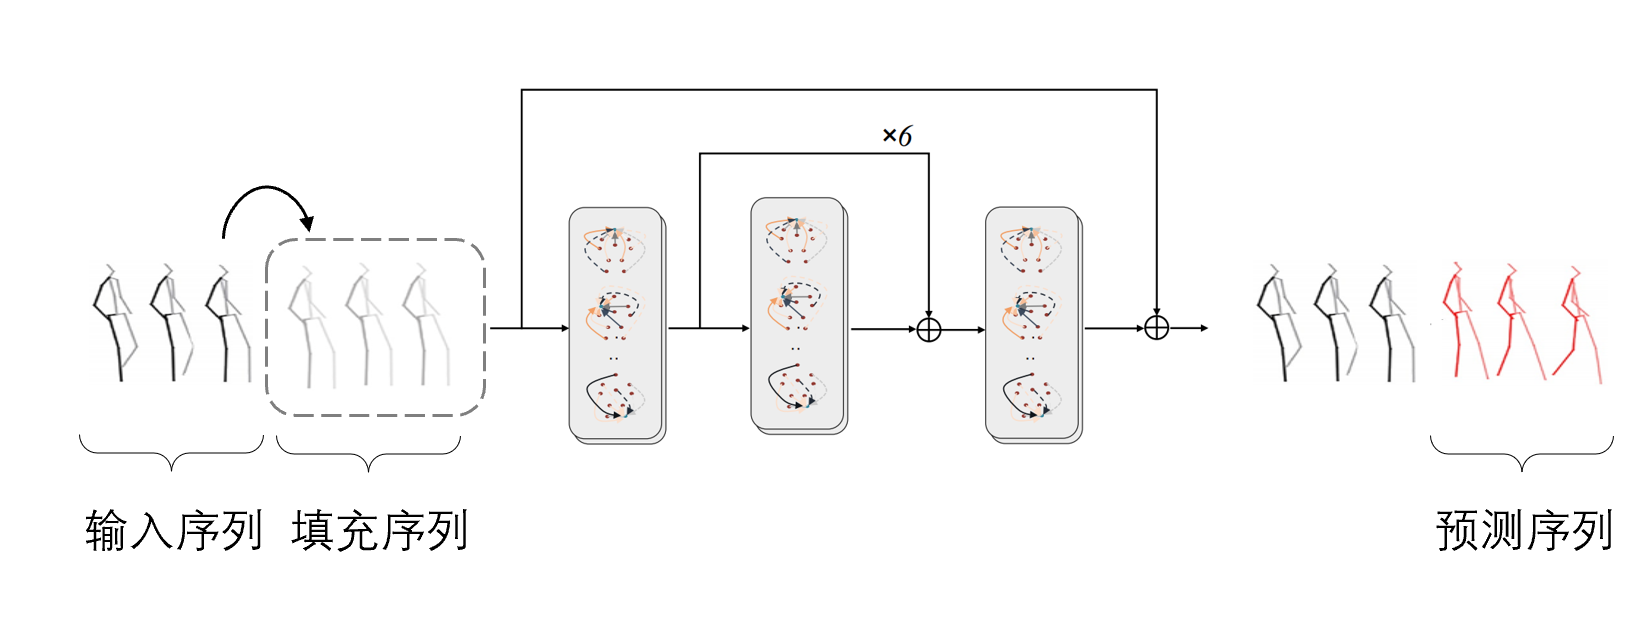
\includegraphics[width=1\textwidth]{FigMa/LTD_padding.png}\\
    \vspace{-0.3cm}
    \caption{LTD数据填充过程}
    \label{fig:LTD_padding}
\end{figure}
然而这种粗糙的填补方法也有其固有缺陷。首先整个填充过程不区分时序距离,全部使用最后一帧进行填充,对于离$P_{T_h}$较近的未来运动,$P_{T_h}$还能提供一定的参考。随着时间向前,未来帧与$P_{T_h}$的关联越来越弱,其提供的参考价值也越来越低,预测的不确定性也逐渐增加。因此该填充方法无法缓解较远距离的预测不确定问题。

LTD证明了通过消除输入数据和预测目标之间的维度差异,可以有效降低预测不确定性。而本文希望验证,缩小二者在内容上的差异也能达到同样的效果。因此,本文以LTD为基准模型,设计了图\ref{fig:toy_experiment}中所示的验证实验。在实验中,预测目标保持不变,输入数据的填充内容被替换为部分预测目标的均值,例如图\ref{fig:toy_experiment}中所表示的真值中前$L$帧的均值。直觉上,填入均值相当于向输入数据泄露了部分预测目标的信息,直接缩短了二者在内容上的差距,进而大幅降低了预测难度。图\ref{fig:toy_experiment}展示的结果也验证了本文的猜想,以均值形式混入的预测目标信息有效缩短了输入数据和预测目标之间的差距,整体预测精度相较于LTD有了明显提升,且混入的信息越多对应位置以及整体上预测精度提升幅度越大。

\begin{figure}[h]
    \centering
    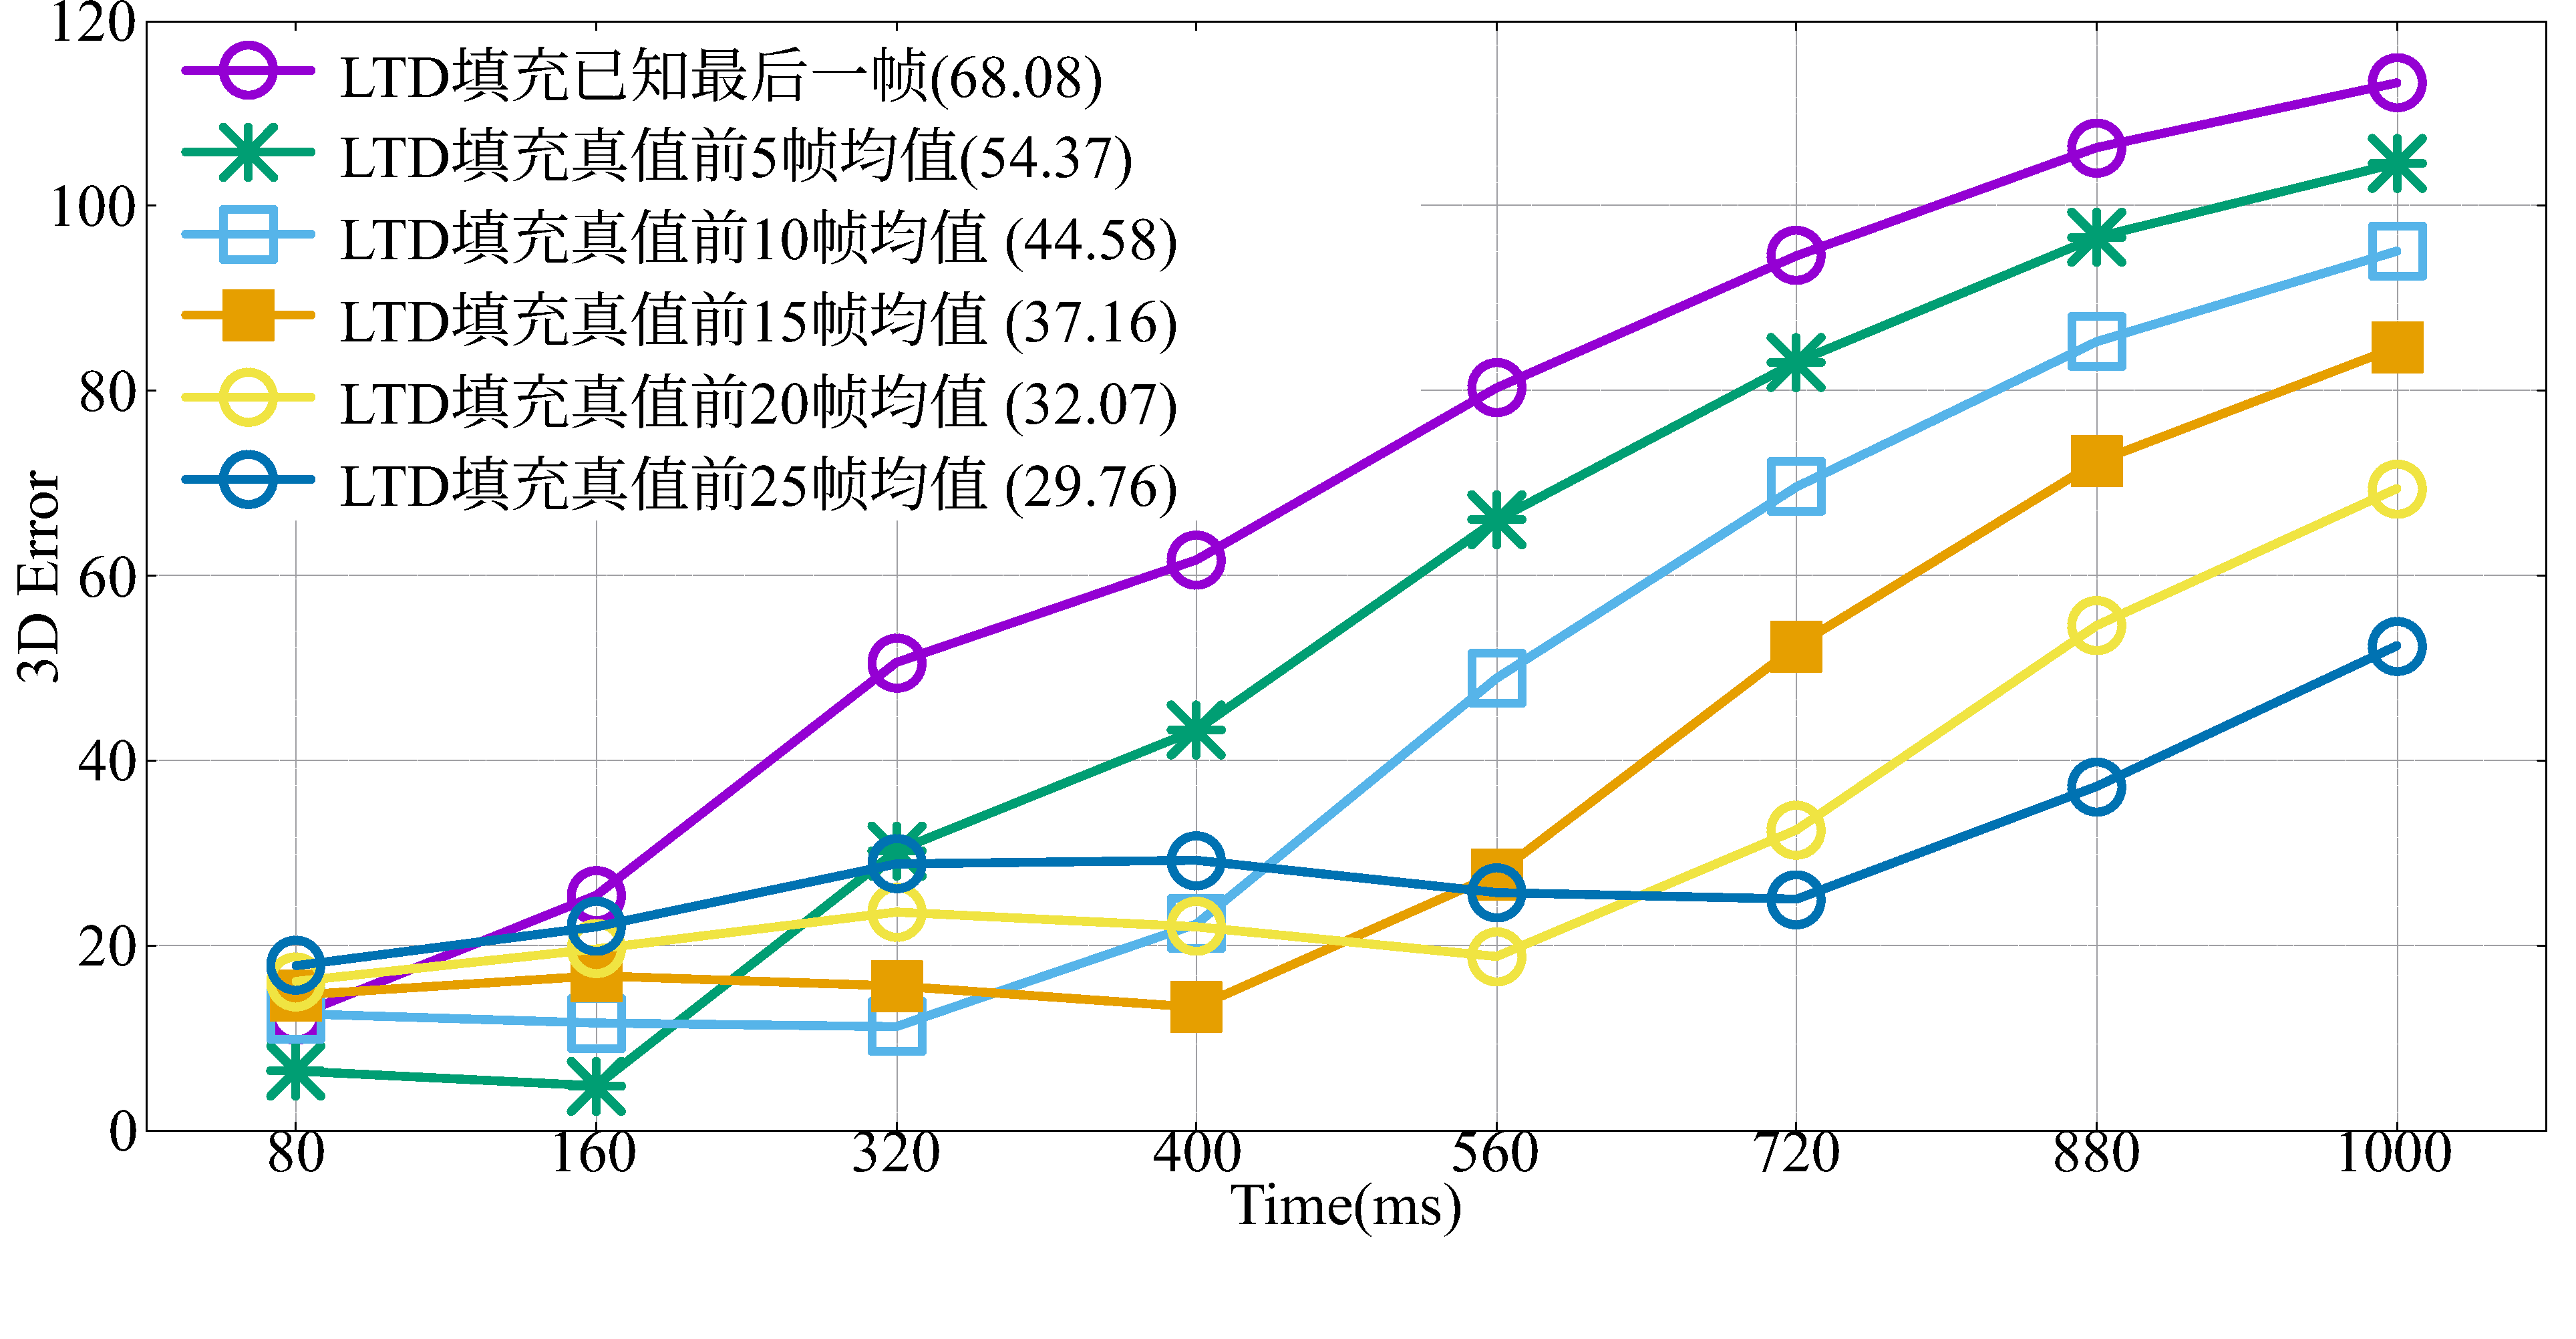
\includegraphics[width=0.8\textwidth]{FigMa/padding_chinese.pdf}\\
    \vspace{-0.3cm}
    \caption{基于LTD的不同内容填充实验}
    \label{fig:toy_experiment}
\end{figure}

\subsection{通过Coarse to fine二阶段网络降低预测不确定性}
在分析上述结果后,本文认为,缩小输入序列和待预测序列的差异(维度差异、内容差异等)可以有效降低预测过程中的不确定性,大幅提高预测的精确性。但将最后一帧作为输入序列的填充,显然并非一个好的选择。如果存在更好的缩小输入序列和目标序列之间差异的方法可以进一步提升预测精度。

由于在实际预测场景中,无法将预测目标信息泄露给输入数据,因此无法参考图\ref{fig:toy_experiment}中的做法,直接使用真值填充输入序列。受到最近被广泛应用的由粗糙到精细(Coarse to fine)策略的启发,本文希望通过分割预测任务,将预测模型分为两个阶段,两个阶段各负责一部分预测任务。由此,每个阶段中,输入和输出数据间的差异被大大缩小。具体的,Coarse to fine 策略与大多数一步到位的方法不同,预测被分为了两个阶段。位于网络浅层的阶段被称为粗糙(Coarse)网络,它接收原始的输入,并输出一个较为粗糙的结果,虽然该结果离最终的目标存在一定的偏差,但与最初的输入信息相比,它已经包含了真值中的绝大部分运动信息。随后该粗糙结果被送入精修(Fine)网络,精修网络将在粗糙网络的基础上进一步完善预测细节。该策略被广泛应用于图片修复(Image Inpainting)\parencite{yu2018generative,zamir2021multi}领域,在该类方法中,原始缺失图片通常由粗糙网络生成一个低分辨率较模糊的修复版本,此次修复的目的是修复图片内容的结构。随后,粗修版本被送入精修网络提高分辨率并进一步完善细节,最后输出高质量的修复结果。参考该思路,本文设计了一个Coarse to fine 人体运动姿态预测网络。

\begin{figure}[ht]
    \centering
    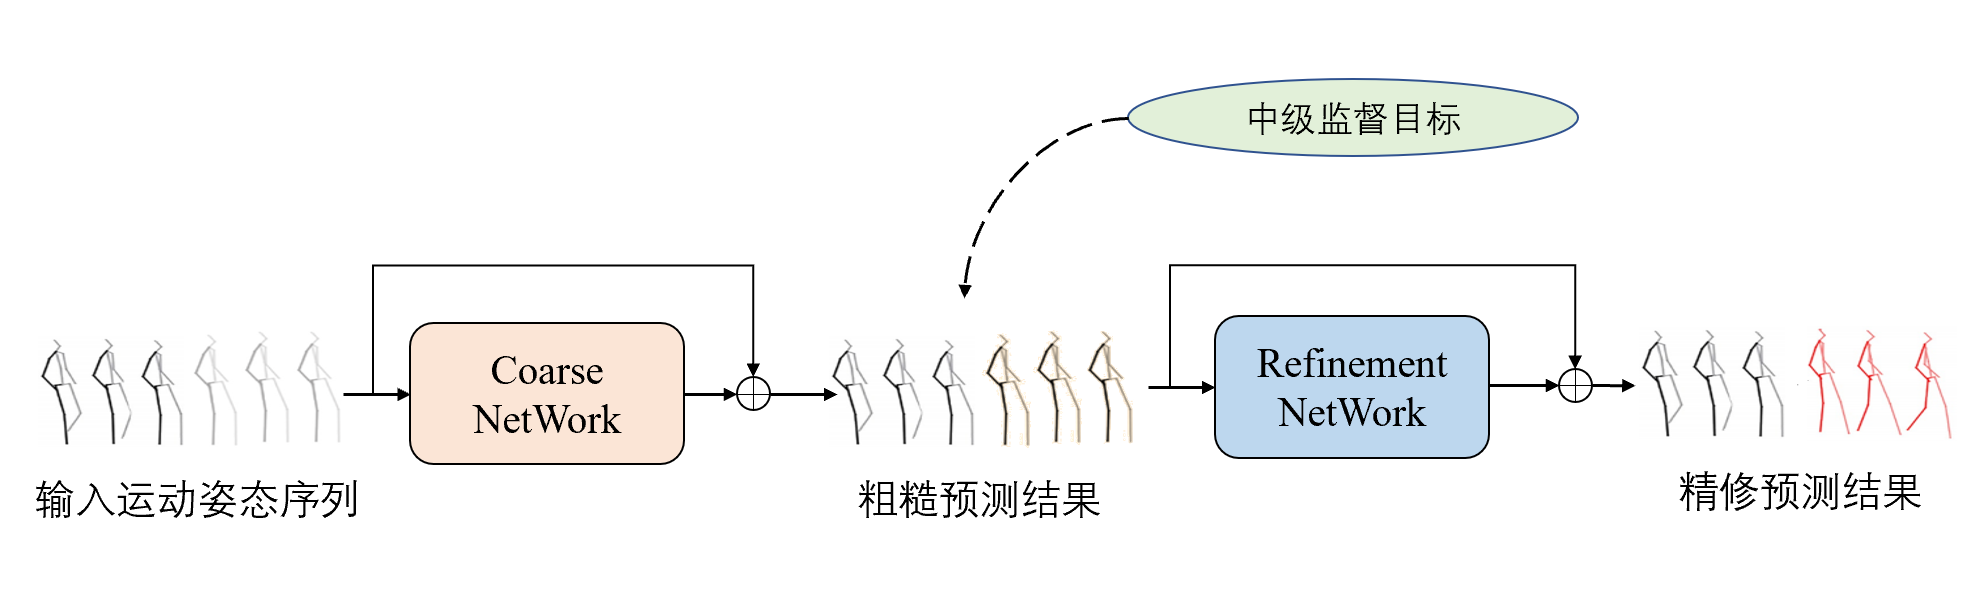
\includegraphics[width=0.8\textwidth]{FigMa/Two_stage.png}\\
    \vspace{-0.3cm}
    \caption{Coarse to fine 二阶段预测网络}
    \label{fig:Two_stage}
\end{figure}

在最初的粗修阶段中,本文任然保留了LTD中基于最后一帧的填充步骤,因为此步骤可以保证网络输入输出维度一致,减少维度上的不确定性。经过填充后的输入序列经过粗修网络,预测得到一个较为粗糙的结果,该结果受到中级监督目标的监督。该中级监督目标相比较最终的预测目标,去除了部分运动细节,只保留了运动大致趋势。随后,粗糙的预测结果被送入后续的精修网络,进一步丰富动作的细节。此时,预测结果受到最终预测目标的监督,以期望获得与真值一致的结果。该模型通过两阶段的结构,将预测过程拆分为两个部分,显著缩小了输入数据和预测目标间的内容差异,大大降低了预测的不确定性。最终,预测精确性与单阶段的LTD网络相比有显著提升(3D预测误差对比:LTD(68.3),Coarse to fine二阶段预测网络(66.9))。
%\subsection{渐进式多阶段预测网络框架}
\subsection{从二阶段网络推广到渐进式多阶段网络}
随后本文进一步拓展了该网络,将一个两阶段的Coarse to fine网络拓展为多阶段的网络。通过对预测过程的进一步细分,每个阶段的预测难度被进一步降低,网络也容易做出准确的预测。本文将多阶段的网络模型定义如下。
\begin{equation}
    \begin{aligned}
         \hat{S}_{1:L}^{1} &= \Phi^1([{S}_{1:T_h};P_{T_h},\cdots,P_{T_h}]), \\
        \hat{S}_{1:L}^{i} &= \Phi^i([S_{1:T_h};\hat{S}_{T_h+1:L}^{i-1}]), i = {2,3,\cdots,T},
    \end{aligned}
    \label{equation:multi-stage_formulation}
\end{equation}
公式\ref{equation:multi-stage_formulation}中,现有方法中单阶段的预测过程$\Phi$被拆分为多个阶段$\Phi = \{ \Phi_1, \cdots, \Phi_T\}$,每个阶段在上一个阶段的预测基础上,不断完善预测精度,使得预测精确度不断稳步提升,相比较现有的单阶段网络,多阶段网络预测过程更加可控,每阶段的预测结构都受到与之对应的中级监督目标的监督,此外预测任务的细分也使得每阶段网络的预测不确定性进一步降低,预测难度也进一步降低。为此,本文设计了一个多阶段的网络,其网络结构图如图\ref{fig:multi_stage}所示。

多阶段的网络设计包含两点,第一是每个阶段(Stage)的子网络设计,在这里本文最初使用了LTD中提出的GCN模块(在文章后续内容中本文提出了具有更强时空信息提取能力的ST-DGCN模块用以替换)。每个子网络内部为一个前馈神经网络网络(Feed forward),。内部由$n$个GCB(GCN Block)构成,每个GCB又由两个GCL(GCN Layer)构成,GCL是网络的最基本的构成结构,其具体结构如图\ref{equation:multi-stage_formulation}右下角所示,GCL由一个GCN、BatchNorm、Tanh和DropOut组成,可以完成最基本的人体运动姿态时空信息提取功能。值得注意的是,网络的规模并不随着阶段数量的增加而提升,在本文的设计中,网络中的GCB数量固定,随着阶段的增加,每个阶段包含的GCB数量等比例下降。
\begin{figure}[ht]
    \centering
    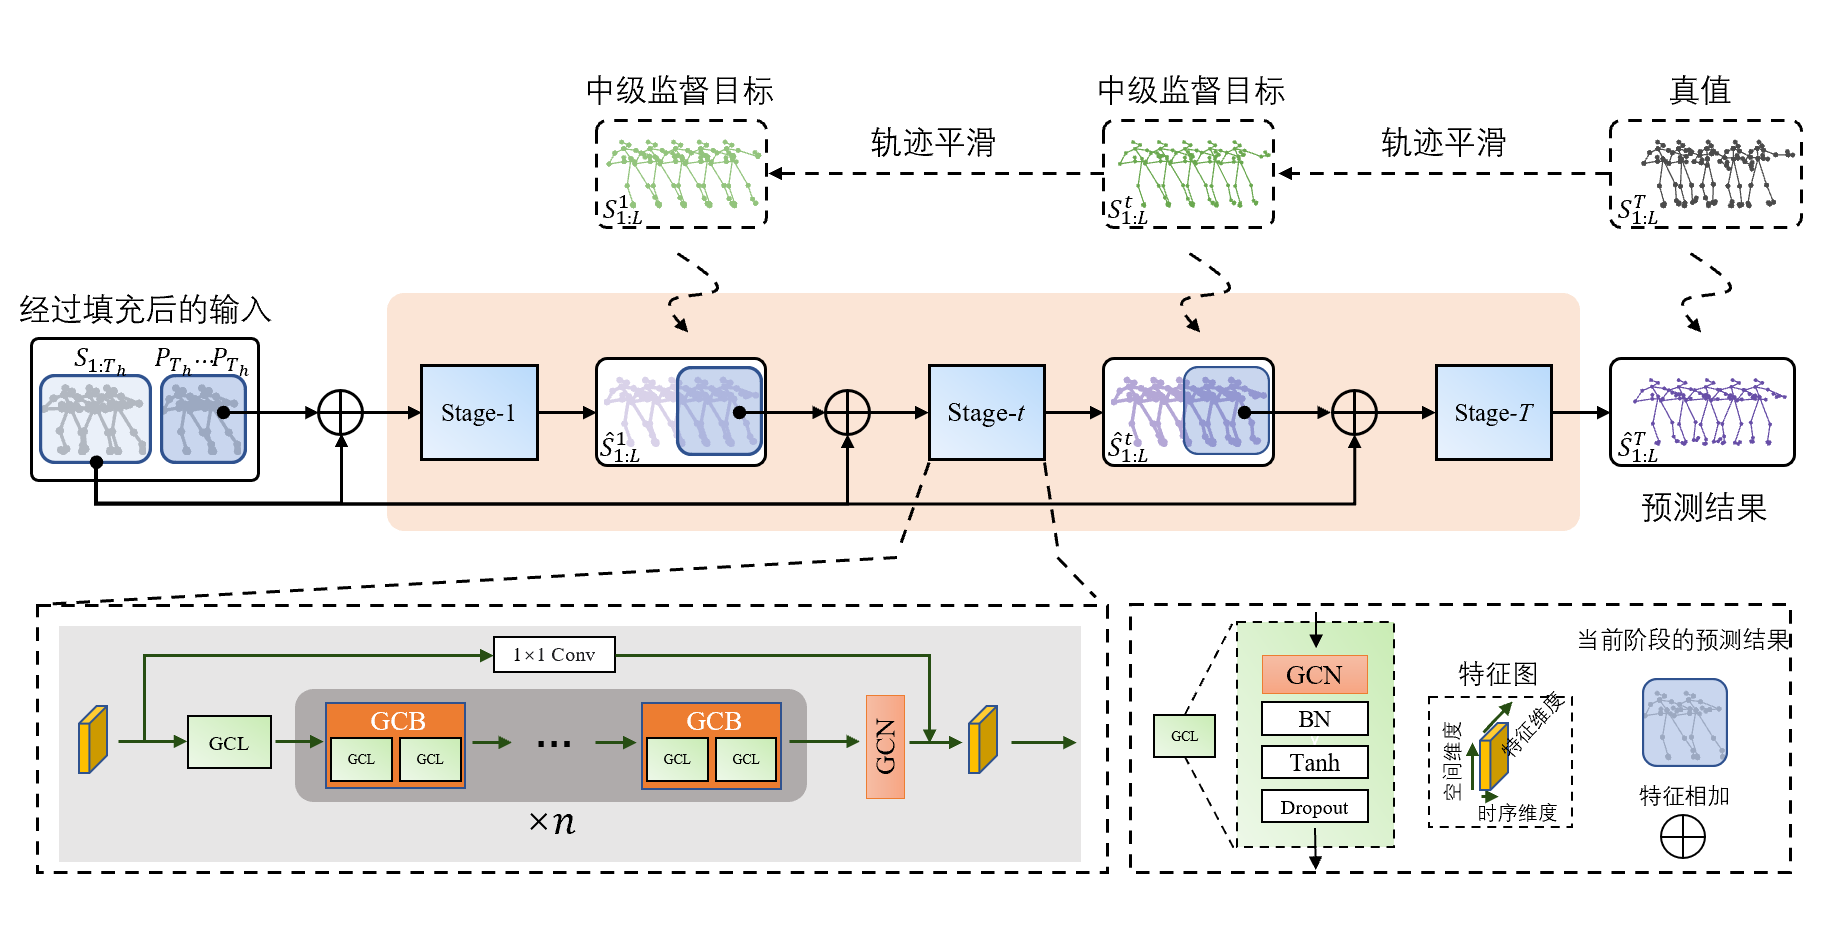
\includegraphics[width=1\textwidth]{FigMa/multi-stage_network.png}\\
    \vspace{-0.3cm}
    \caption{渐进式多阶段的预测网络}
    \label{fig:multi_stage}
\end{figure}
网络参数量的增加在一定范围下提高了网络的容量和表达能力,但当突破某一阈值的时候网络复杂度增加带来的计算开销负担抵消了这一优势。本文的多阶段网络,通过控制网络中的GCB数量,在提升网络性能的同时,维持了网络规模基本不变。
第二点是中级监督目标的设计,中级监督目标必须具有层次化特点,遵循由简单到复杂的原则,浅层网络负责较为简单的整体运动趋势预测,而深层网络负责较为复杂的细节完善任务。在其他类型任务(图像等规则数据)的中级监督目标设计中,可以简单地通过降低分辨率、模糊处理和提取边缘特征等方式降低图片的细节或提取内容的结构信息来构造中级监督目标。但人体运动姿态数据是不规则的拓扑数据。无法通过寻常的降维手段提取结构信息或降低运动复杂度。虽然当前也有一些方法,如MSR\parencite{dang2021msr}提出在空间维度上对人体结构进行降维,合并运动模型类似的相邻关节点来减少图中的关节点数量,构造具有空间层次结构的中级监督目标。但该方法破坏了重要的人体结构先验信息,抵消了渐进式多阶段策略对网络性能的提升。

\subsection{渐进式多阶段网络中的中级监督目标构造方法}
本文设计了一种适用于人体运动姿态数据的中级监督目标构建方法,该方法可以在保持原有的空间结构的同时,降低时间维度上的关节点运动复杂度。具体的,本文在不同阶段对关节点轨迹施加不同强度的平滑算法作为中级监督目标。网络浅层因为表达能力不足,因此其对应的中级监督目标被施加了更强的平滑来降低运动的复杂度和预测难度。随着网络深入,网络的表达能力增加,能够承担更复杂的预测任务。此时,对于中级监督目标的平滑程度就会被削弱,以帮助其在之前阶段的预测基础上,丰富运动细节。为此,本文设计了一种名为累积均值平滑(Accumulated Average Smoothing)的方法构造用于人体运动姿态序列预测问题的中级监督目标。

在介绍累积均值平滑算法之前,为了方便叙述,本文首先给出人体运动姿态模型中关节点轨迹的数学定义。假设每个人体姿态包含$V$个关节点,每个关节点由$D$维的向量描述。一个人体运动姿态序列$S_{1:L}$包含$V \times D$条轨迹:$\{T_j|j\in[1, M\times D]\}$,每条轨迹$T_j$由同一个关节点的某位维度上的运动组成:$T_j=\{x^i_j|i\in[1,L]\}$。由于所有轨迹都由同样的平滑方法处理,在下面的叙述中本文忽略了不同轨迹的区别,统一用$T$代称$T_j$。

$T$由两部分组成:已知的运动序列$\{x^i|i\in[1,T_h]\}$和待预测的运动序列$\{x^i|i\in[T_h+1,T_h+T_f]\}$。由于已知的运动序列属于模型的输入数据,不需要预测,所以不需要经过累积平滑算法处理。待预测的真实运动序列则需要用累积平滑算法调节该部分数据的预测难度。目前被广泛使用的平滑方式是基于高斯卷积核的滤波器。高斯滤波器被广泛应用于图像平滑领域,它是一种常见的线性滤波器。它的原理是将一个二维高斯分布函数应用于图像的每一个像素,使得该像素周围的像素加权平均起来,从而达到平滑图像的目的。高斯滤波器的核心是高斯核(Gaussian kernel),也称为卷积核(Convolution Kernel)或滤波器(Filter)。高斯核是一个二维高斯分布函数,它的中心是图像上的当前像素点。高斯核中的每个元素表示该位置的权重,越靠近中心位置的像素权重越高,越远离中心位置的像素权重越低。通常情况下,高斯核是一个奇数×奇数的矩阵,这样可以保证中心像素的位置。在轨迹平滑算法中,2D的高斯卷积核退化为1D,其卷积核权重计算公式为:
\begin{equation}
    G(x) = \frac{1}{\sqrt{2\pi}\sigma}e^{-\frac{x^2}{2\sigma^2}}
    \label{equation:gauss_filter}
\end{equation}
其中$x$表示当前位置相对于卷积核中心的距离,$\sigma$表示标准差,标准差越大越靠近卷积核中心的权重越高,反之权重分布越平均。
\begin{equation}
    G = \frac{1}{\sqrt{2\pi}\sigma}
        \begin{bmatrix}e^{-\frac{-{((N-1)/2)} ^2}{2\sigma^2}} & \cdots & e^{-\frac{-{((N-1)/2)}^2}{2\sigma^2}} \\ 
        \vdots & \ddots & \vdots \\
        e^{-\frac{0^2}{2\sigma^2}} & \cdots & e^{-\frac{0^2}{2\sigma^2}} \\
        \vdots & \ddots & \vdots \\
        e^{-\frac{{((N-1)/2)}^2}{2\sigma^2}} & \cdots & e^{-\frac{{((N-1)/2)}^2}{2\sigma^2}
        }\end{bmatrix}
    \label{equation:gauss_filter_mat}
\end{equation}
如果需要生成一个$N\times 1$的高斯卷积核,可以通过上述公式\ref{equation:gauss_filter}得到卷积核矩阵\ref{equation:gauss_filter_mat},其中,$G$ 是 $N\times 1$ 的高斯卷积核矩阵,$N$ 表示卷积核的大小。

由于在本问题中,只需要对一条轨迹待预测部分进行平滑,已知的运动序列保持不变即可。而高斯滤波器在对轨迹进行处理时,不可避免地计算卷积核范围内的所有数据,因此在已知运动序列和待预测部分的过渡部分会出现跳跃(Jump)现象,这是由于高斯滤波器在计算过渡部分的平滑值时,将卷积核范围内已知运动序列纳入计算。而已知运动序列在最终的结果中并没有被平滑,所以导致计算结果在该处出现了跳跃现象。此外,由于高斯滤波器在计算时,其节点原始值的权重较高,导致平滑力度不足,难以构造层次化的中级监督目标。

因此,本文提出了累积均值平滑算法来解决以上两个问题。本文将该算法定义如下:

\begin{equation}
    \bar{x}^i = \frac{1}{i-T_h}\sum_{k=T_h+1}^{i}x^k, \forall i\in[T_h+1, T_h+T_f].
    \label{equation:AAS}
\end{equation}

待预测部分的某个节点的平滑值由其之前所有节点的累计平均值得到。首先平滑值计算过程只涉及待预测部分,不涉及已知部分,这就避免了出现过渡部分的跳跃问题。其次,该节点的平滑值是由前面所有节点的平均值而非加权平均得出的。这意味着每个节点在平滑过程中都具有相等的影响力,没有任何一个节点能够主导结果。这种方法消除了原始节点权重过高,影响平滑效果的问题。另外,随着当前节点离已知部分的距离增加,该参与平滑计算的节点数量也逐渐增加,平滑力度也随之增强。这符合一般直觉,距离已知部分较远的节点预测难度更大,需要更强的平滑力度来降低预测难度。相反,靠近已知部分的节点保留了更多的原始信息,这是因为这些节点的不确定性较低,预测难度也相对较低,因此不需要进行过度平滑。因此,该算法能够基于每个节点的不确定性程度和预测难度来自适应地平衡平滑力度和原始信息保留。这使得该算法可以在处理各种复杂的预测问题时,提供具有层次化,且更合理的中级监督目标。总之,累积均值平滑算法相比传统的高斯滤波算法能够生成过渡更平滑,难度梯度更合理的中级监督目标,能有效地帮助网络建立一个渐进式的学习框架,降低预测难度,提高网络学习效率。

\begin{figure}[ht]
    \centering
    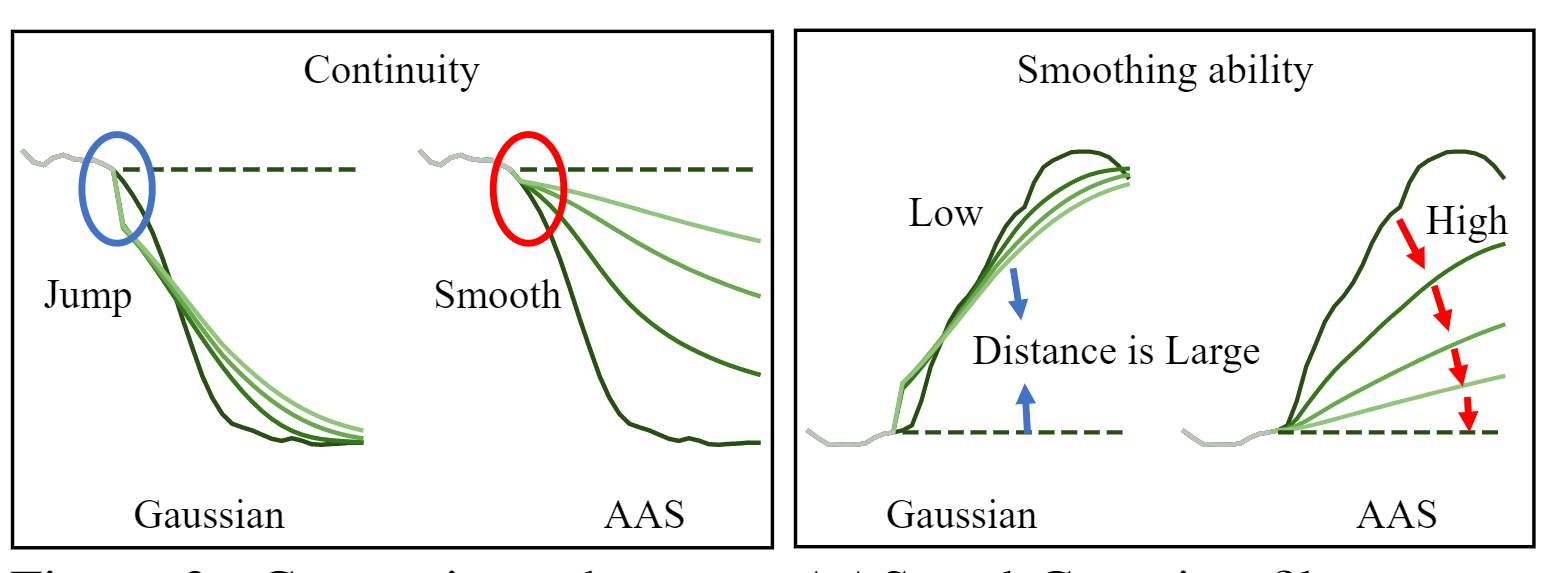
\includegraphics[width=1\textwidth]{FigMa/AAS.png}\\
    \vspace{-0.3cm}
    \caption{累积均值平滑对比高斯滤波}
    \label{fig:AAS}
\end{figure}
上图展示了累积均值平滑算法(AAS)和高斯滤波算法(Gaussian)的平滑结果对比。其中灰色实线是输入模型的已知运动序列,深绿色虚线是使用已知运动序列最后一帧构成的填充序列。接下来由深到浅的绿色实线是不同阶段的平滑结果。拥有最深颜色的曲线是待预测的真实运动序列,稍浅一点的为经过一次平滑的结果,后续逐渐变浅的线段是经过多次平滑的结果,颜色越浅则经历的平滑次数越多。

图\ref{fig:AAS}左展示了高斯滤波出现的过渡部分跳跃问题。从图中可以看到,待预测的真实轨迹与已知序列的过渡部分是平滑的。然而在经过高斯滤波处理后,平滑后的待预测轨迹与已知部分的连接处,出现了明显的跳跃现象,这是由于在计算该部分平滑值时,卷积核窗口包含了已知序列和待预测序列两部分的信息。而本文提出的累积均值平滑算法解决了这一问题,在对某个节点进行平滑处理时,纳入计算的运动数据只涉及当前节点之前的待预测运动序列,不包含已知运动序列,且平滑的强度随时间增加而线性增长。例如,当计算待预测序列的第一个节点的平滑值时,由于该节点已经位于待预测序列的开始位置,因此,计算该节点的平滑值只需将该节点代入公式\ref{equation:AAS},得到的结果也既是它本身。由于平滑节点数据未发生突变,因此可以和已知部分平滑过渡。

图\ref{fig:AAS}右,展示了累积均值平滑算法和高斯滤波算法的平滑力度对比。在高斯滤波算法的计算过程中,卷积核窗口给予了当前节点过高的权重,导致平滑结果与当前节点的差异较小。最终,即使在经过迭代后的多次平滑步骤。最终结果的平滑程度仍然较低,无法满足构造层次化的中级监督目标的要求。而在累积均值平滑算法中,采用了累积的策略,越远离已知部分的节点受到的平滑力度越大,其次,使用平均的计算方法而不是加权平均的算法,平滑结果受到原始数据的影响更小,平滑的结果也更加明显。累积均值平滑算法的平滑结果表明,该算法能够在去除信号噪声的同时,保留数据序列的趋势特征。与其他常见的平滑算法相比,累积均值平滑算法在平滑强度方面表现更加优秀。这种层次化的特点使得累积均值平滑算法的平滑结果更加符合渐进式策略中预测目标由易到难的变化趋势,为多阶段预测网络模型提供了更好的中间监督目标。该中间监督目标可以有效地降低预测难度,并提高预测的准确性和稳定性。因此,基于累积均值平滑算法的平滑结果是一种有价值的中间监督目标,它可以帮助多阶段预测网络模型实现更加准确、稳定和可靠的预测结果。

\subsection{总结}
本章介绍了基于渐进式策略的多阶段人体运动姿态预测网络,以及对应渐进式多阶段网络结构的中级监督目标构造方法。首先本文从对现有方法的分析入手,发现现阶段人体运动姿态预测问题的难点在于输入数据和待预测数据之间的差异过大,导致网络预测过程存在不确定性。LTD提出使用已知部分来填充空白维度,使得输出输出数据达成维度上的统一,消除由于维度差异带来的不确定性。受此启发,本文希望更近一步,通过降低二者在内容上的差异性来消除预测不确定性。为此本文首先设计了一个Coarse to fine二阶段实验网络,人体运动姿态预测被分为两个部分,第一个阶段网络的预测目标是较简单的大致的运动趋势,第二阶段的网络在上一步的基础上完善复杂的运动细节,使最终的网络输出与真值一致。在两阶段的网络中,本文在不增加网络参数量的前提下,通过分解任务的方式将缩小了各个阶段中,输入与输出之间内容上的差距,从而降低了预测的不确定性。在最终的设计中,本文将两阶段的网络推广到多阶段的网络,进一步体现渐进式策略的优势。

本文的另一个贡献点是提出了一种名为累积均值平滑的中级监督目标构造方法,该方法相比较常用的高斯滤波平滑方法,可以避免平滑后运动序列的过渡部分出现跳跃现象。此外,由于其累积平滑的特性,拥有更强的平滑能力,相比高斯滤波平滑能够生成更具层次化的中级监督目标,辅助多阶段网络构建一个从难到易的网络预测框架。

除了通过基于渐进式策略的多阶段网络结构来降低输入数据和预测目标内容上的差距,本文还期望提高网络中的基础图卷积模块的时空信息提取能力,来降低预测过程的不确定性。现有图卷积模块或缺失了对时序信息的建模,或感受野范围受限于传统算子的卷积核大小,又或是带来了不可接受的网络规模膨胀。而本文希望提出一种在不显著提升时空开销的前提下,拥有对时空信息高效建模能力的GCN模块。本文将在下一节详细阐述该方案。
	% \include{chapter01}%第一章
	\include{chapter02}%第二章
	\include{chapter03}%第三章
	\include{chapter04}
	% 自行根据需要添加章节。

	\backmatter %章节不编号但页码继续
	%%%%%%%%%%%%%%%%%%%%%%%%%%%%%%%%%%%%%%%%%%%%%%%%%%%%%%%%%%%%%%    微调,使得后续章节的页眉不带章号——by MCH
	\renewcommand{\chaptermark}[1]{\markboth{#1}{}}
	%%%%%%%%%%%%%%%%%%%%%%%%%%%%%%%%%%%%%%%%%%%%%%%%%%%%%%%%%%%%%%
	\chapter{总结与展望}
人体运动姿态序列预测算法近十年在学术界和工业界都得到了广泛的研究,该算法可以被应用于国民经济信息化、智能化建设的方方面面,例如自动驾驶、智能机器人、人机交互和多媒体领域。而当前在这该算法上的研究受限于预测过程中的不确定性和特征提取算子时空信息提取能力的缺失,在预测精度和执行效率方面任然存在不足。本文在充分调研和分析现有方法后提出了一种名为“基于渐进式策略的人体运动姿态预测算法”来解决上述问题。

具体的,本方法有两点创新,第一,针对复杂长时人体运动姿态预测过程中不确定性大的问题。本文提出使用渐进式策略,设计一个多阶段网络,将整体的预测任务分割为多个子任务,每个阶段只需要在上一个阶段的基础上进行预测。整个预测过程遵循由难到易的原则,浅层网络只负责预测运动的大致趋势,而具体末端运动细节则由后续深层网络在此基础上完善。在多阶段网络模型中,中级监督目标的设计尤为重要。由于人体运动姿态数据属于不规则图数据,难以像图像一样可以简单地进行下采样。因此,本文提出了名为累积均值平滑的中级监督目标构造方法。在该方法中,本文保留了重要的空间结构先验信息,通过平滑关节点轨迹的方式降低运动的复杂程度。相比较基于高斯卷积核的平滑方法,该方法能避免过渡部分的不连续,提供更加具有层次化的中级监督目标,辅助不同阶段间的预测平滑过渡。

第二,针对现有特征提取算子时空信息捕捉能力弱的缺点,本文提出了一种新的图卷积模块称为ST-DGCN,该模块由两个串联的GCN构成,分别被称为S-DGCN和T-DGCN,前者负责处理空间上人体结构信息,后者负责处理时间维度上的关节点运动信息。训练时,特征首先通过S-DGCN被提取空间信息,随后被送入T-DGCN提取时间信息,网络由此间接地感知到了人体运动姿态序列中的时空特征。与现有特征提取算子相比,ST-DGCN通过时空分离和参数共享的形式降低了网络参数量,由于时间和空间维度均使用图卷积进行建模,网络在时空都具有全局感受野,拥有对时空长时依赖的建模能力。

随后本文通过详细的定性和定量实验分析,证明了本方法在预测精确度和时空效率两方面都领先现有先进方法。随后的消融实验证明了本文的多阶段网络相比较现有的单阶段预测方法有较大的优势。ST-DGCN图卷积模块也优于现有的特征提取算子。综上,本文提出了基于渐进式策略的人体运动姿态预测算法在预测精确度和时空效率两个指标上全面领先现有方法,显著推动了该领域相关问题的研究进展。

但本方法也存在一些未解决的问题,可以作为未来的拓展研究方向。首先,在人体运动姿态序列预测问题中,预测的上限由输入数据中的信息决定,如果输入运动序列和待预测的运动序列之间的差距过大,或是待预测的运动序列过长,即使将输入序列中的有效信息完全利用也无法有效降低预测过程中的不确定性。在这种情况下片面追求预测的精确性已经成为了一个不可能完成的任务。近来一些生成式的方法为该问题提供了解决思路,它们通过在预测过程中添加一定的随机性,可以在接受同一个输入序列的情况下,生成多个不同的未来运动序列。该类方法不再片面追求预测的精确性,而是兼顾预测结果真实性。

当前研究的另一个不足,是缺乏一个对结果客观评估的度量指标,现有指标MPJPE计算预测关节点与真实关节点间的平均误差,作为度量预测质量的标准。然而该方法对所有关节点一视同仁,无法反映关节点之间的差异(一般来说,本文更关注运动模式复杂的末端关节点,而不是运动平稳躯干关节点)。目前有部分方法采用了主观评价或基于判别器的方法,为解决这个问题提供了新思路。 %结论
	 %%%%%%%%%%%%%%%%%%%%%%%%%%%%%%%%%%%%%%%%%%%%%% bibtex参考文献设置  (原版)
%%	\bibliographystyle{scutthesis}
%%	\bibliography{F:/MyLibrary}
	%%%%%%%%%%%%%%%%%%%%%%%%%%%%%%%%%%%%%%%%%%%%%%
	%%%%%%%%%%%%%%%%%%%%%%%%%%%%%%%%%%%%%%%%%%%%%% biber参考文献设置	——by MCH
	%\renewcommand*{\bibfont}{\refbodyfont}			% 设置文献著录字号比正文小一号(五号),需要小四号请注释该行. % 不推荐使用small,而是使用cls文件中精确定义了的字号。
	\phantomsection % “目录”中的链接能正确跳转,需要添加 \phantomsection 否则点击参考文献会跳转到结论
	\addcontentsline{toc}{chapter}{参考文献}	%目录中添加参考文献
	\printbibliography	% 参考文献著录
 	%%%%%%%%%%%%%%%%%%%%%%%%%%%%%%%%%%%%%%%%%%%%%%
 	% 只有一个附录
% 	\include{appendix}
 	% 有多个附录
	\include{appendix1} %附录1
	\include{appendix2} %附录2
 	%%%%%%%%%%%%%%%%%%%
	\chapter{攻读博士/硕士学位期间取得的研究成果} %博士/硕士记得选其一
\pubfont % 论文撰写规范里,这章是5号宋体,\pubfont 设置字号为5号了。但其实很多论文用小四号也OK。
一、已发表(包括已接受待发表)的论文,以及已投稿、或已成文打算投稿、或拟成文投稿的论文情况\underline{\textbf{(只填写与学位论文内容相关的部分):}}
\begin{table}
	\centering{}%
	\pubfont 
	\begin{longtable}{|>{\centering}m{0.5cm}|m{1.8cm}|>{\centering}m{2.8cm}|>{\centering}m{2.5cm}|>{\centering}m{2.2cm}|>{\centering}m{2.cm}|>{\centering}m{1cm}|}
		\hline 
		\textbf{序号} & \textbf{作者(全体作者,按顺序排列)} & \textbf{题 目} 						   & \textbf{发表或投稿刊物名称、级别} & \textbf{发表的卷期、年月、页码} & \textbf{与学位论文哪一部分(章、节)相关} &\textbf{被索引收录情况}\tabularnewline
		\hline 
		1    & 马铁铮、聂勇伟、龙成江、张青、李桂清& Progressively generating better initial guesses towards next stages for high-quality human motion prediction & Proceedings of the IEEE/CVF Conference on Computer Vision and Pattern Recognition(CCF A类会议)& 已录用,2022年3月,页码6437--6446 & 第四章、第五章 & EI\tabularnewline
		\hline 
	\end{longtable}
\end{table}

注:在“发表的卷期、年月、页码”栏:

1.如果论文已发表,请填写发表的卷期、年月、页码;

2.如果论文已被接受,填写将要发表的卷期、年月;

3.以上都不是,请据实填写“已投稿”,“拟投稿”。

不够请另加页。

二、与学位内容相关的其它成果(包括专利、著作、获奖项目等)



%注:这部分一言难尽,我努力了很久都没有把这个表做好。感觉学校给的这个表的模板非常反人类。看国外大学的博士论文,那种像参考文献著录信息那样一行一行的,比较美观。而这个框框很难放文字进去。

\normalsize % \normalsize可以将下文调回和正文一样的字号,这个随个人喜好。注释掉的话,致谢就就跟随《攻读博士/硕士学位期间取得的研究成果》的字号。 %成果
	\chapter{致\texorpdfstring{\quad}{}谢}
%把下面文字替换
在即将完成研究生学业之际,我非常荣幸能够向各位老师和同学们表达我最深刻的感激之情。在这段时间里,您们给予了我无私的指导和关心,让我能够在学术和生活上都得到了莫大的帮助。特别是我的导师聂勇伟副教授,在我的研究方向、论文的思路和实现等方面给予了我深入的指导和帮助,使我得以更好地了解所研究领域的知识,提高了我的研究能力,开拓了我的学术视野。我将永远珍视您对我的帮助和支持,您的辛勤付出将成为我一生中不断前行的动力。

同时,我也要感谢华南理工大学计算机学院的各位老师和同学们。感谢您们在学术、生活和事业上的帮助和鼓励,感谢您们给予我的指导和支持。在学习和生活的过程中,我遇到了许多挑战和困难,但是有您们的陪伴和鼓励,我才能够克服这些困难,不断向前。

此外,我还要感谢我的家人和朋友们。他们一直是我人生道路上的坚实后盾,他们的支持和鼓励是我前进的动力。在我研究生生涯中,他们无私的付出和关爱让我倍感温暖和感激,我会时刻珍惜这份感情。

最后,我要感谢我的朋友们张军,胡益畅,陈海斌,刘知安。感谢他们在学习和生活中的支持和帮助,他们的陪伴让我的研究生生活更加充实而有意义。

再次感谢你们,是你们的支持和帮助让我走到了今天的成就。我会永远铭记你们的谆谆教诲和关心,不断努力学习和提高自己,在自己的岗位上为社会和人民做出更多的贡献。
%把上面文字替换

~\\

\begin{minipage}[t]{0.945\textwidth}%
	\begin{flushright}
		马铁铮\\
%		\today\\	% 自动时间
		2022年6月10日\\	%固定时间
		于华南理工大学
		\par\end{flushright}
\end{minipage}

 %致谢
\end{document}
